% Autor: Gabriel Costa Fassarella
% Data: 16/03/2023
% UENF - CCT - LCMAT - C.Computação 
% Prof. Ausberto Castro
% Disciplina: Paradigmas de Linguagem de Programação
%%%---------------------------------------------

\documentclass[12pt,fleqn]{book} % Default font size and left-justified equations

%----------------------------------------------------------------------------------------

%%%%%%%%%%%%%%%%%%%%%%%%%%%%%%%%%%%%%%%%%
% The Legrand Orange Book 
% Structural Definitions File
% Version 2.0 (9/2/15)
%
% Original author:
% Mathias Legrand (legrand.mathias@gmail.com) with modifications by:
% Vel (vel@latextemplates.com)
%
% This file has been downloaded from:
% http://www.LaTeXTemplates.com
%
% License: 
% CC BY-NC-SA 3.0 (http://creativecommons.org/licenses/by-nc-sa/3.0/)
%
%%%%%%%%%%%%%%%%%%%%%%%%%%%%%%%%%%%%%%%%%%

%----------------------------------------------------------------------------------------
%	VARIOUS REQUIRED PACKAGES AND CONFIGURATIONS
%----------------------------------------------------------------------------------------

\usepackage[top=3cm,bottom=3cm,left=3cm,right=3cm,headsep=10pt,a4paper]{geometry} % Page margins

\usepackage{graphicx} % Required for including pictures
\graphicspath{{Pictures/}} % Specifies the directory where pictures are stored

\usepackage{lipsum} % Inserts dummy text
\usepackage{here}   %
\usepackage{tikz} % Required for drawing custom shapes

\usepackage[brazil]{babel} % Brazilian Portuguese language/hyphenation

\usepackage{enumitem} % Customize lists
\setlist{nolistsep} % Reduce spacing between bullet points and numbered lists

\usepackage{booktabs} % Required for nicer horizontal rules in tables

\usepackage{xcolor} % Required for specifying colors by name
\definecolor{ocre}{RGB}{243,102,25} % Define the orange color used for highlighting throughout the book

\usepackage{bibentry}
%----------------------------------------------------------------------------------------
%	FONTS
%----------------------------------------------------------------------------------------

\usepackage{avant} % Use the Avantgarde font for headings
%\usepackage{times} % Use the Times font for headings
\usepackage{mathptmx} % Use the Adobe Times Roman as the default text font together with math symbols from the Sym­bol, Chancery and Com­puter Modern fonts

\usepackage{microtype} % Slightly tweak font spacing for aesthetics
\usepackage[utf8]{inputenc} % Required for including letters with accents
\usepackage[T1]{fontenc} % Use 8-bit encoding that has 256 glyphs

%----------------------------------------------------------------------------------------
%	BIBLIOGRAPHY AND INDEX
%----------------------------------------------------------------------------------------
\usepackage{hyperref}



\sloppy




%\usepackage[style=alphabetic, citestyle=numeric, sorting=nyt, sortcites=true,
%            autopunct=true, babel=hyphen, hyperref=true, abbreviate=false,
%            backref=true, backend=biber]{biblatex}
%\addbibresource{racketbib.bib} % BibTeX bibliography file
%\defbibheading{bibempty}{}

\usepackage{calc} % For simpler calculation - used for spacing the index letter headings correctly
\usepackage{makeidx} % Required to make an index
\makeindex % Tells LaTeX to create the files required for indexing

%----------------------------------------------------------------------------------------
%	MAIN TABLE OF CONTENTS
%----------------------------------------------------------------------------------------

\usepackage{titletoc} % Required for manipulating the table of contents

\contentsmargin{0cm} % Removes the default margin

% Part text styling
\titlecontents{part}[0cm]
{\addvspace{20pt}\centering\large\bfseries}
{}
{}
{}

% Chapter text styling
\titlecontents{chapter}[1.25cm] % Indentation
{\addvspace{12pt}\large\sffamily\bfseries} % Spacing and font options for chapters
{\color{ocre!60}\contentslabel[\Large\thecontentslabel]{1.25cm}\color{ocre}} % Chapter number
{\color{ocre}}
{\color{ocre!60}\normalsize\;\titlerule*[.5pc]{.}\;\thecontentspage} % Page number

% Section text styling
\titlecontents{section}[1.25cm] % Indentation
{\addvspace{3pt}\sffamily\bfseries} % Spacing and font options for sections
{\contentslabel[\thecontentslabel]{1.25cm}} % Section number
{}
{\hfill\color{black}\thecontentspage} % Page number
[]

% Subsection text styling
\titlecontents{subsection}[1.25cm] % Indentation
{\addvspace{1pt}\sffamily\small} % Spacing and font options for subsections
{\contentslabel[\thecontentslabel]{1.25cm}} % Subsection number
{}
{\ \titlerule*[.5pc]{.}\;\thecontentspage} % Page number
[]

% List of figures
\titlecontents{figure}[0em]
{\addvspace{-5pt}\sffamily}
{\thecontentslabel\hspace*{1em}}
{}
{\ \titlerule*[.5pc]{.}\;\thecontentspage}
[]

% List of tables
\titlecontents{table}[0em]
{\addvspace{-5pt}\sffamily}
{\thecontentslabel\hspace*{1em}}
{}
{\ \titlerule*[.5pc]{.}\;\thecontentspage}
[]

%----------------------------------------------------------------------------------------
%	MINI TABLE OF CONTENTS IN PART HEADS
%----------------------------------------------------------------------------------------

% Chapter text styling
\titlecontents{lchapter}[0em] % Indenting
{\addvspace{15pt}\large\sffamily\bfseries} % Spacing and font options for chapters
{\color{ocre}\contentslabel[\Large\thecontentslabel]{1.25cm}\color{ocre}} % Chapter number
{}
{\color{ocre}\normalsize\sffamily\bfseries\;\titlerule*[.5pc]{.}\;\thecontentspage} % Page number

% Section text styling
\titlecontents{lsection}[0em] % Indenting
{\sffamily\small} % Spacing and font options for sections
{\contentslabel[\thecontentslabel]{1.25cm}} % Section number
{}
{}

% Subsection text styling
\titlecontents{lsubsection}[.5em] % Indentation
{\normalfont\footnotesize\sffamily} % Font settings
{}
{}
{}

%----------------------------------------------------------------------------------------
%	PAGE HEADERS
%----------------------------------------------------------------------------------------

\usepackage{fancyhdr} % Required for header and footer configuration

\pagestyle{fancy}
\renewcommand{\chaptermark}[1]{\markboth{\sffamily\normalsize\bfseries\chaptername\ \thechapter.\ #1}{}} % Chapter text font settings
\renewcommand{\sectionmark}[1]{\markright{\sffamily\normalsize\thesection\hspace{5pt}#1}{}} % Section text font settings
\fancyhf{} \fancyhead[LE,RO]{\sffamily\normalsize\thepage} % Font setting for the page number in the header
\fancyhead[LO]{\rightmark} % Print the nearest section name on the left side of odd pages
\fancyhead[RE]{\leftmark} % Print the current chapter name on the right side of even pages
\renewcommand{\headrulewidth}{0.5pt} % Width of the rule under the header
\addtolength{\headheight}{2.5pt} % Increase the spacing around the header slightly
\renewcommand{\footrulewidth}{0pt} % Removes the rule in the footer
\fancypagestyle{plain}{\fancyhead{}\renewcommand{\headrulewidth}{0pt}} % Style for when a plain pagestyle is specified

% Removes the header from odd empty pages at the end of chapters
\makeatletter
\renewcommand{\cleardoublepage}{
\clearpage\ifodd\c@page\else
\hbox{}
\vspace*{\fill}
\thispagestyle{empty}
\newpage
\fi}

%----------------------------------------------------------------------------------------
%	THEOREM STYLES
%----------------------------------------------------------------------------------------

\usepackage{amsmath,amsfonts,amssymb,amsthm} % For math equations, theorems, symbols, etc

\newcommand{\intoo}[2]{\mathopen{]}#1\,;#2\mathclose{[}}
\newcommand{\ud}{\mathop{\mathrm{{}d}}\mathopen{}}
\newcommand{\intff}[2]{\mathopen{[}#1\,;#2\mathclose{]}}
\newtheorem{notation}{Notation}[chapter]

% Boxed/framed environments
\newtheoremstyle{ocrenumbox}% % Theorem style name
{0pt}% Space above
{0pt}% Space below
{\normalfont}% % Body font
{}% Indent amount
{\small\bf\sffamily\color{ocre}}% % Theorem head font
{\;}% Punctuation after theorem head
{0.25em}% Space after theorem head
{\small\sffamily\color{ocre}\thmname{#1}\nobreakspace\thmnumber{\@ifnotempty{#1}{}\@upn{#2}}% Theorem text (e.g. Theorem 2.1)
\thmnote{\nobreakspace\the\thm@notefont\sffamily\bfseries\color{black}---\nobreakspace#3.}} % Optional theorem note
\renewcommand{\qedsymbol}{$\blacksquare$}% Optional qed square

\newtheoremstyle{blacknumex}% Theorem style name
{5pt}% Space above
{5pt}% Space below
{\normalfont}% Body font
{} % Indent amount
{\small\bf\sffamily}% Theorem head font
{\;}% Punctuation after theorem head
{0.25em}% Space after theorem head
{\small\sffamily{\tiny\ensuremath{\blacksquare}}\nobreakspace\thmname{#1}\nobreakspace\thmnumber{\@ifnotempty{#1}{}\@upn{#2}}% Theorem text (e.g. Theorem 2.1)
\thmnote{\nobreakspace\the\thm@notefont\sffamily\bfseries---\nobreakspace#3.}}% Optional theorem note

\newtheoremstyle{blacknumbox} % Theorem style name
{0pt}% Space above
{0pt}% Space below
{\normalfont}% Body font
{}% Indent amount
{\small\bf\sffamily}% Theorem head font
{\;}% Punctuation after theorem head
{0.25em}% Space after theorem head
{\small\sffamily\thmname{#1}\nobreakspace\thmnumber{\@ifnotempty{#1}{}\@upn{#2}}% Theorem text (e.g. Theorem 2.1)
\thmnote{\nobreakspace\the\thm@notefont\sffamily\bfseries---\nobreakspace#3.}}% Optional theorem note

% Non-boxed/non-framed environments
\newtheoremstyle{ocrenum}% % Theorem style name
{5pt}% Space above
{5pt}% Space below
{\normalfont}% % Body font
{}% Indent amount
{\small\bf\sffamily\color{ocre}}% % Theorem head font
{\;}% Punctuation after theorem head
{0.25em}% Space after theorem head
{\small\sffamily\color{ocre}\thmname{#1}\nobreakspace\thmnumber{\@ifnotempty{#1}{}\@upn{#2}}% Theorem text (e.g. Theorem 2.1)
\thmnote{\nobreakspace\the\thm@notefont\sffamily\bfseries\color{black}---\nobreakspace#3.}} % Optional theorem note
\renewcommand{\qedsymbol}{$\blacksquare$}% Optional qed square
\makeatother

% Defines the theorem text style for each type of theorem to one of the three styles above
\newcounter{dummy}
\numberwithin{dummy}{section}
\theoremstyle{ocrenumbox}
\newtheorem{theoremeT}[dummy]{Theorem}
\newtheorem{problem}{Problem}[chapter]
\newtheorem{exerciseT}{Exercise}[chapter]
\theoremstyle{blacknumex}
\newtheorem{exampleT}{Example}[chapter]
\theoremstyle{blacknumbox}
\newtheorem{vocabulary}{Vocabulary}[chapter]
\newtheorem{definitionT}{Definition}[section]
\newtheorem{corollaryT}[dummy]{Corollary}
\theoremstyle{ocrenum}
\newtheorem{proposition}[dummy]{Proposition}

%----------------------------------------------------------------------------------------
%	DEFINITION OF COLORED BOXES
%----------------------------------------------------------------------------------------

\RequirePackage[framemethod=default]{mdframed} % Required for creating the theorem, definition, exercise and corollary boxes

% Theorem box
\newmdenv[skipabove=7pt,
skipbelow=7pt,
backgroundcolor=black!5,
linecolor=ocre,
innerleftmargin=5pt,
innerrightmargin=5pt,
innertopmargin=5pt,
leftmargin=0cm,
rightmargin=0cm,
innerbottommargin=5pt]{tBox}

% Exercise box	
\newmdenv[skipabove=7pt,
skipbelow=7pt,
rightline=false,
leftline=true,
topline=false,
bottomline=false,
backgroundcolor=ocre!10,
linecolor=ocre,
innerleftmargin=5pt,
innerrightmargin=5pt,
innertopmargin=5pt,
innerbottommargin=5pt,
leftmargin=0cm,
rightmargin=0cm,
linewidth=4pt]{eBox}	

% Definition box
\newmdenv[skipabove=7pt,
skipbelow=7pt,
rightline=false,
leftline=true,
topline=false,
bottomline=false,
linecolor=ocre,
innerleftmargin=5pt,
innerrightmargin=5pt,
innertopmargin=0pt,
leftmargin=0cm,
rightmargin=0cm,
linewidth=4pt,
innerbottommargin=0pt]{dBox}	

% Corollary box
\newmdenv[skipabove=7pt,
skipbelow=7pt,
rightline=false,
leftline=true,
topline=false,
bottomline=false,
linecolor=gray,
backgroundcolor=black!5,
innerleftmargin=5pt,
innerrightmargin=5pt,
innertopmargin=5pt,
leftmargin=0cm,
rightmargin=0cm,
linewidth=4pt,
innerbottommargin=5pt]{cBox}

% Creates an environment for each type of theorem and assigns it a theorem text style from the "Theorem Styles" section above and a colored box from above
\newenvironment{theorem}{\begin{tBox}\begin{theoremeT}}{\end{theoremeT}\end{tBox}}
\newenvironment{exercise}{\begin{eBox}\begin{exerciseT}}{\hfill{\color{ocre}\tiny\ensuremath{\blacksquare}}\end{exerciseT}\end{eBox}}				
\newenvironment{definition}{\begin{dBox}\begin{definitionT}}{\end{definitionT}\end{dBox}}	
\newenvironment{example}{\begin{exampleT}}{\hfill{\tiny\ensuremath{\blacksquare}}\end{exampleT}}		
\newenvironment{corollary}{\begin{cBox}\begin{corollaryT}}{\end{corollaryT}\end{cBox}}	

%----------------------------------------------------------------------------------------
%	REMARK ENVIRONMENT
%----------------------------------------------------------------------------------------

\newenvironment{remark}{\par\vspace{10pt}\small % Vertical white space above the remark and smaller font size
\begin{list}{}{
\leftmargin=35pt % Indentation on the left
\rightmargin=25pt}\item\ignorespaces % Indentation on the right
\makebox[-2.5pt]{\begin{tikzpicture}[overlay]
\node[draw=ocre!60,line width=1pt,circle,fill=ocre!25,font=\sffamily\bfseries,inner sep=2pt,outer sep=0pt] at (-15pt,0pt){\textcolor{ocre}{R}};\end{tikzpicture}} % Orange R in a circle
\advance\baselineskip -1pt}{\end{list}\vskip5pt} % Tighter line spacing and white space after remark

%----------------------------------------------------------------------------------------
%	SECTION NUMBERING IN THE MARGIN
%----------------------------------------------------------------------------------------

\makeatletter
\renewcommand{\@seccntformat}[1]{\llap{\textcolor{ocre}{\csname the#1\endcsname}\hspace{1em}}}
\renewcommand{\section}{\@startsection{section}{1}{\z@}
{-4ex \@plus -1ex \@minus -.4ex}
{1ex \@plus.2ex }
{\normalfont\large\sffamily\bfseries}}
\renewcommand{\subsection}{\@startsection {subsection}{2}{\z@}
{-3ex \@plus -0.1ex \@minus -.4ex}
{0.5ex \@plus.2ex }
{\normalfont\sffamily\bfseries}}
\renewcommand{\subsubsection}{\@startsection {subsubsection}{3}{\z@}
{-2ex \@plus -0.1ex \@minus -.2ex}
{.2ex \@plus.2ex }
{\normalfont\small\sffamily\bfseries}}
\renewcommand\paragraph{\@startsection{paragraph}{4}{\z@}
{-2ex \@plus-.2ex \@minus .2ex}
{.1ex}
{\normalfont\small\sffamily\bfseries}}

%----------------------------------------------------------------------------------------
%	PART HEADINGS
%----------------------------------------------------------------------------------------

% numbered part in the table of contents
\newcommand{\@mypartnumtocformat}[2]{%
\setlength\fboxsep{0pt}%
\noindent\colorbox{ocre!20}{\strut\parbox[c][.7cm]{\ecart}{\color{ocre!70}\Large\sffamily\bfseries\centering#1}}\hskip\esp\colorbox{ocre!40}{\strut\parbox[c][.7cm]{\linewidth-\ecart-\esp}{\Large\sffamily\centering#2}}}%
%%%%%%%%%%%%%%%%%%%%%%%%%%%%%%%%%%
% unnumbered part in the table of contents
\newcommand{\@myparttocformat}[1]{%
\setlength\fboxsep{0pt}%
\noindent\colorbox{ocre!40}{\strut\parbox[c][.7cm]{\linewidth}{\Large\sffamily\centering#1}}}%
%%%%%%%%%%%%%%%%%%%%%%%%%%%%%%%%%%
\newlength\esp
\setlength\esp{4pt}
\newlength\ecart
\setlength\ecart{1.2cm-\esp}
\newcommand{\thepartimage}{}%
\newcommand{\partimage}[1]{\renewcommand{\thepartimage}{#1}}%
\def\@part[#1]#2{%
\ifnum \c@secnumdepth >-2\relax%
\refstepcounter{part}%
\addcontentsline{toc}{part}{\texorpdfstring{\protect\@mypartnumtocformat{\thepart}{#1}}{\partname~\thepart\ ---\ #1}}
\else%
\addcontentsline{toc}{part}{\texorpdfstring{\protect\@myparttocformat{#1}}{#1}}%
\fi%
\startcontents%
\markboth{}{}%
{\thispagestyle{empty}%
\begin{tikzpicture}[remember picture,overlay]%
\node at (current page.north west){\begin{tikzpicture}[remember picture,overlay]%	
\fill[ocre!20](0cm,0cm) rectangle (\paperwidth,-\paperheight);
\node[anchor=north] at (4cm,-3.25cm){\color{ocre!40}\fontsize{220}{100}\sffamily\bfseries\@Roman\c@part};
\node[anchor=south east] at (\paperwidth-1cm,-\paperheight+1cm){\parbox[t][][t]{8.5cm}{
\printcontents{l}{0}{\setcounter{tocdepth}{1}}%
}};
\node[anchor=north east] at (\paperwidth-1.5cm,-3.25cm){\parbox[t][][t]{15cm}{\strut\raggedleft\color{white}\fontsize{30}{30}\sffamily\bfseries#2}};
\end{tikzpicture}};
\end{tikzpicture}}%
\@endpart}
\def\@spart#1{%
\startcontents%
\phantomsection
{\thispagestyle{empty}%
\begin{tikzpicture}[remember picture,overlay]%
\node at (current page.north west){\begin{tikzpicture}[remember picture,overlay]%	
\fill[ocre!20](0cm,0cm) rectangle (\paperwidth,-\paperheight);
\node[anchor=north east] at (\paperwidth-1.5cm,-3.25cm){\parbox[t][][t]{15cm}{\strut\raggedleft\color{white}\fontsize{30}{30}\sffamily\bfseries#1}};
\end{tikzpicture}};
\end{tikzpicture}}
\addcontentsline{toc}{part}{\texorpdfstring{%
\setlength\fboxsep{0pt}%
\noindent\protect\colorbox{ocre!40}{\strut\protect\parbox[c][.7cm]{\linewidth}{\Large\sffamily\protect\centering #1\quad\mbox{}}}}{#1}}%
\@endpart}
\def\@endpart{\vfil\newpage
\if@twoside
\if@openright
\null
\thispagestyle{empty}%
\newpage
\fi
\fi
\if@tempswa
\twocolumn
\fi}

%----------------------------------------------------------------------------------------
%	CHAPTER HEADINGS
%----------------------------------------------------------------------------------------

\newcommand{\thechapterimage}{}%
\newcommand{\chapterimage}[1]{\renewcommand{\thechapterimage}{#1}}%
\def\@makechapterhead#1{%
{\parindent \z@ \raggedright \normalfont
\ifnum \c@secnumdepth >\m@ne
\if@mainmatter
\begin{tikzpicture}[remember picture,overlay]
\node at (current page.north west)
{\begin{tikzpicture}[remember picture,overlay]
\node[anchor=north west,inner sep=0pt] at (0,0) {\includegraphics[width=\paperwidth]{\thechapterimage}};
\draw[anchor=west] (\Gm@lmargin,-9cm) node [line width=2pt,rounded corners=15pt,draw=ocre,fill=white,fill opacity=0.5,inner sep=15pt]{\strut\makebox[22cm]{}};
\draw[anchor=west] (\Gm@lmargin+.3cm,-9cm) node {\huge\sffamily\bfseries\color{black}\thechapter. #1\strut};
\end{tikzpicture}};
\end{tikzpicture}
\else
\begin{tikzpicture}[remember picture,overlay]
\node at (current page.north west)
{\begin{tikzpicture}[remember picture,overlay]
\node[anchor=north west,inner sep=0pt] at (0,0) {\includegraphics[width=\paperwidth]{\thechapterimage}};
\draw[anchor=west] (\Gm@lmargin,-9cm) node [line width=2pt,rounded corners=15pt,draw=ocre,fill=white,fill opacity=0.5,inner sep=15pt]{\strut\makebox[22cm]{}};
\draw[anchor=west] (\Gm@lmargin+.3cm,-9cm) node {\huge\sffamily\bfseries\color{black}#1\strut};
\end{tikzpicture}};
\end{tikzpicture}
\fi\fi\par\vspace*{270\p@}}}

%-------------------------------------------

\def\@makeschapterhead#1{%
\begin{tikzpicture}[remember picture,overlay]
\node at (current page.north west)
{\begin{tikzpicture}[remember picture,overlay]
\node[anchor=north west,inner sep=0pt] at (0,0) {\includegraphics[width=\paperwidth]{\thechapterimage}};
\draw[anchor=west] (\Gm@lmargin,-9cm) node [line width=2pt,rounded corners=15pt,draw=ocre,fill=white,fill opacity=0.5,inner sep=15pt]{\strut\makebox[22cm]{}};
\draw[anchor=west] (\Gm@lmargin+.3cm,-9cm) node {\huge\sffamily\bfseries\color{black}#1\strut};
\end{tikzpicture}};
\end{tikzpicture}
\par\vspace*{270\p@}}
\makeatother

%----------------------------------------------------------------------------------------
%	HYPERLINKS IN THE DOCUMENTS
%----------------------------------------------------------------------------------------

\usepackage{hyperref}
\hypersetup{hidelinks,backref=true,pagebackref=true,hyperindex=true,colorlinks=false,breaklinks=true,urlcolor= ocre,bookmarks=true,bookmarksopen=false,pdftitle={Title},pdfauthor={Author}}
\usepackage{bookmark}
\bookmarksetup{
open,
numbered,
addtohook={%
\ifnum\bookmarkget{level}=0 % chapter
\bookmarksetup{bold}%
\fi
\ifnum\bookmarkget{level}=-1 % part
\bookmarksetup{color=ocre,bold}%
\fi
}
}

%----------------------------------------------------------------------------------------
\usepackage[many]{tcolorbox}
\tcbset{skin=enhanced}


\usepackage{listings}
         \lstset{ %
  	      language={Scala}, % % lenguaje de programaci\'{o}n
  	      basicstyle=\bfseries\ttfamily,
  	      keywordstyle=\color{blue},
  	      commentstyle=\color{brown},	
  	      backgroundcolor=\color{green!10},
  	      showstringspaces=false
  	      }

%----------------------------------------------------------------------------------------
\usepackage[brazilian,hyperpageref]{backref}
% Configura\c{c}\~{o}es do pacote backref
% Usado sem a op\c{c}\~{a}o hyperpageref de backref
\renewcommand{\backrefpagesname}{Citado na(s) p\'{a}gina(s):~}
% Texto padr\~{a}o antes do n\'{u}mero das p\'{a}ginas
\renewcommand{\backref}{}
% Define os textos da cita\c{c}\~{a}o
\renewcommand*{\backrefalt}[4]{
	\ifcase #1 %
		Nenhuma cita\c{c}\~{a}o no texto.%
	\or
		Citado na p\'{a}gina #2.%
	\else
		Citado #1 vezes nas p\'{a}ginas #2.%
	\fi}%
% ---
%----------------------------------------------------------------------------------------
\hypersetup{
    bookmarks=true,         % show bookmarks bar?
    unicode=false,          % non-Latin characters in Acrobat’s bookmarks
    pdftoolbar=true,        % show Acrobat’s toolbar?
    pdfmenubar=true,        % show Acrobat’s menu?
    pdffitwindow=true,     % window fit to page when opened
    pdfstartview={FitH},    % fits the width of the page to the window
    pdftitle={Tutorial sobre a Linguagem Fortran},    % title
  %  pdfauthor={Mariana A. Gualhano and Ausberto S. Castro Vera},     % author
    pdfsubject={Paradigmas de Linguagens de Programa\c{c}\~{a}o},   % subject of the document
    pdfcreator={ASCV, WinEdt},   % creator of the document
    pdfproducer={ASCV}, % producer of the document
    pdfkeywords={Programa\c{c}\~{a}o} {Imperativo} {Paradigmas}, % list of keywords
    pdfnewwindow=true,      % links in new window
    colorlinks=true,       % false: boxed links; true: colored links
    linkcolor=red,          % color of internal links (change box color with linkbordercolor)
    citecolor=blue,        % color of links to bibliography
    filecolor=magenta,      % color of file links
    urlcolor=cyan           % color of external links
}	
 % Insert the commands.tex file which contains the majority of the structure behind the template

\begin{document}

%----------------------------------------------------------------------------------------
%	TITLE PAGE
%----------------------------------------------------------------------------------------

\begingroup
\thispagestyle{empty}
\begin{tikzpicture}[remember picture,overlay]
\coordinate [below=12cm] (midpoint) at (current page.north);
\node at (current page.north west)
{\begin{tikzpicture}[remember picture,overlay]
\node[anchor=north west,inner sep=0pt] at (0,0)
        {
\includegraphics[width=\paperwidth]{capa.png}}; %Capa Imagem A4 21x29.7
\draw[anchor=north] (midpoint) node [fill=ocre!30!white,fill opacity=0.6,text opacity=1,inner sep=1cm]{\Huge\centering\bfseries\sffamily\parbox[c][][t]
        {\paperwidth}
        {\centering Introdu\c{c}\~{a}o \`{a} Linguagem Scala\\[5pt] % Titulo Livro
{\Large Paradigmas de Linguagens de Programa\c{c}\~{a}o}\\[20pt] % Subtitle
{\huge   \color{blue} Gabriel Costa Fassarella}\\ % Autor nome
{\huge  \color{blue}  Ausberto S. Castro Vera}\\
{\small \today}
}}; % Autor nome
\end{tikzpicture}};
\end{tikzpicture}
\vfill

\endgroup

%----------------------------------------------------------------------------------------
%	COPYRIGHT PAGE
%----------------------------------------------------------------------------------------

\newpage
% Prof. Dr. Ausberto S. Castro Vera
% UENF - CCT - LCMAT - Curso de Ci\^{e}ncia da Computa\c{c}\~{a}o
% Campos, RJ,  2023
% Disciplina: Paradigmas de Linguagens de Programa\c{c}\~{a}o
% Aluno: Gabriel Costa Fassarella




\noindent
\textbf{Disciplina:} \textit{Paradigmas de Linguagens de Programa\c{c}\~{a}o 2023}\\
\textbf{Linguagem:} \textit{Scala}\\
\textbf{Aluno:} \textit{ \color{blue} Gabriel Costa Fassarella}


\section*{Ficha de avalia\c{c}\~{a}o:}



\begin{tabular}{|p{12cm}|c|}
  \hline
  % after \\: \hline or \cline{col1-col2} \cline{col3-col4} ...
  \textbf{Aspectos de avalia\c{c}\~{a}o (requisitos m\'{\i}nimos)} & \textbf{Pontos} \\
  \hline
   \color{red} Introdu\c{c}\~{a}o (M\'{a}ximo: 01 pontos) &  \\
  $\bullet$ Aspectos hist\'{o}ricos &  \\
  $\bullet$ \'{A}reas de Aplica\c{c}\~{a}o da linguagem &  \\
  \hline
 \color{red}  Elementos b\'{a}sicos da linguagem (M\'{a}ximo: 01 pontos) &  \\
  $\bullet$ Sintaxe (vari\'{a}veis, constantes, comandos, opera\c{c}\~{o}es, etc.) &  \\
  $\bullet$ Cada elemento com exemplos (c\'{o}digo e execu\c{c}\~{a}o) &  \\
  \hline
  \color{red} Aspectos Avan\c{c}ados da linguagem (M\'{a}ximo: 2,0 pontos) &  \\
  $\bullet$ Sintaxe (vari\'{a}veis, constantes, comandos, opera\c{c}\~{o}es, etc.) &  \\
  $\bullet$ Cada elemento com exemplos (c\'{o}digo e execu\c{c}\~{a}o) &  \\
  $\bullet$ Exemplos com fonte diferenciada (listing) & \\
  \hline
  \color{red} M\'{\i}nimo 5 Aplica\c{c}\~{o}es completas - Aplica\c{c}\~{o}es (M\'{a}ximo : 2,0 pontos) &  \\
  $\bullet$ Uso de rotinas-fun\c{c}\~{o}es-procedimentos, E/S formatadas &  \\
  $\bullet$ Uma Calculadora &  \\
  $\bullet$ Gr\'{a}ficos &  \\
  $\bullet$ Algoritmo QuickSort &  \\
  $\bullet$ Outra aplica\c{c}\~{a}o &  \\
  $\bullet$ Outras aplica\c{c}\~{o}es ... &  \\
  \hline
  \color{red} Ferramentas (compiladores, interpretadores, etc.) (M\'{a}ximo : 1,0 pontos) &  \\
  $\bullet$ Ferramentas utilizadas nos exemplos: pelo menos DUAS&  \\
  $\bullet$ Descri\c{c}\~{a}o de Ferramentas existentes:  m\'{a}ximo 5&  \\
  $\bullet$ Mostrar as telas dos exemplos junto ao compilador-interpretador&  \\
  $\bullet$ Mostrar as telas dos resultados com o uso das ferramentas &  \\
  $\bullet$ Descri\c{c}\~{a}o das ferramentas (autor, vers\~{a}o, homepage, tipo, etc.) &  \\
  \hline
  \color{red} Organiza\c{c}\~{a}o do trabalho (M\'{a}ximo: 01 ponto) &  \\
  $\bullet$ Conte\'{u}do, Historia, Se\c{c}\~{o}es, gr\'{a}ficos, exemplos, conclus\~{o}es, bibliografia &  \\
  $\bullet$ Cada elemento com exemplos (c\'{o}digo e execu\c{c}\~{a}o, ferramenta, nome do aluno) &  \\
  \hline
  \color{red} Uso de Bibliografia (M\'{a}ximo: 01 ponto)&  \\
   $\bullet$ Livros: pelo menos 3&  \\
   $\bullet$ Artigos cient\'{\i}ficos: pelo menos 3 (IEEE Xplore, ACM Library)&  \\
   $\bullet$ Todas as Refer\^{e}ncias dentro do texto, tipo [ABC 04] & \\
   $\bullet$ Evite Refer\^{e}ncias da Internet & \\
   \hline
     &  \\
  \color{red} Conceito do Professor (Opcional: 01 ponto) & \\
  \hline
   & \\
  \hfill \color{blue} Nota Final do trabalho: & \\
  \hline
\end{tabular}\\
\textit{Observa\c{c}\~{a}o:} Requisitos m\'{\i}nimos significa a \textit{metade} dos pontos

\newpage
~\vfill

\thispagestyle{empty}

\noindent Copyright \copyright\  \the\year{} Gabriel Costa Fassarella e Ausberto S. Castro Vera\\ % Copyright notice

\noindent \textsc{UENF - Universidade Estadual do Norte Fluminense Darcy Ribeiro}\\ % Universidade

\noindent \textsc{CCT - Centro de Ci\^{e}ncia e Tecnologia}\\ % Centro
\noindent \textsc{LCMAT - Laborat\'{o}rio de Matem\'{a}ticas}\\ % Laboratorio
\noindent \textsc{CC - Curso de Ci\^{e}ncia da Computa\c{c}\~{a}o}\\ % Curso

%\input{autor.tex} \\

\noindent \textit{Primeira edi\c{c}\~{a}o, Abril 2023} % Printing/edition date

%----------------------------------------------------------------------------------------
%	TABLE OF CONTENTS
%----------------------------------------------------------------------------------------

\chapterimage{sumario01.jpg} % Table of contents heading image

\pagestyle{empty} % No headers

\addtocontents{toc}{\protect{\pdfbookmark[0]{\contentsname}{toc}}}
\tableofcontents % Print the table of contents itself

\cleardoublepage % Forces the first chapter to start on an odd page so it's on the right

\pagestyle{fancy} % Print headers again

%----------------------------------------------------------------------------------------
%	PART
%----------------------------------------------------------------------------------------
%\part{Part One}

%----------------------------------------------------------------------------------------
%	CHAPTERS
%----------------------------------------------------------------------------------------
% Prof. Dr. Ausberto S. Castro Vera
% UENF - CCT - LCMAT - Curso de Ci\^{e}ncia da Computa\c{c}\~{a}o
% Campos, RJ,  2023
% Disciplina: An\'{a}lise e Projeto de Sistemas
% Aluno:


\chapterimage{sistemas.png} % Table of contents heading image
\chapter{ Introdu\c{c}\~{a}o}

Análise de projeto de sistemas é uma disciplina da área da ciências da computação e engenharia de software responsável por se concentrar no processo de desenvolvimento de sistemas computacionais. Abordando desde a compreensão dos requisitos necessários para o sistema, a criação dos modelos e a definição de estruturas para a construção de um software funcional. 

Neste documento será apresentado o sistema D.S.S - Delivery Status System, esse sistema é possível ser aplicado tanto por empresas de entregas internacionais, como por aplicativos de delivery de refeições, aprimorando a logística da empresa assim proporcionando uma melhor experiência ao cliente. Durante esse capítulo será abordada uma descrição do sistema e sua ideia, assim como os principais componentes que garantem a ele um funcionamento adequado.

 \section{Descri\c{c}\~{a}o do Sistema Computacional a desenvolver}
 
 	O início do século XXI proporcionou ao mundo inúmeras mudanças na área da tecnologia, a principal foi a popularização da internet nas casas de grande parte da população mundial. Esse cenário foi capaz de dar um grande "boom" nas interações internacionais, visto que com a internet as relações entre indivíduos extremamente distantes passou a ser cada vez mais fácil de ocorrer. Além disso, a internet se mostrou uma grande ferramenta para o comércio mundial, visto que no mundo contemporâneo, se torna cada vez mais fácil efetuar compras de produtos de outros países, assim como também ocorre em compras locais, como em pedidos por meio de aplicativos de entregas de refeição por exemplo. 
 	
 	Com a evolução da tecnologia e a elevação nas taxas de pedidos por todo o mundo, torna-se necessário a criação de um sistema computacional eficiente de rastreamento de entregas em tempo real que ajude na eficiência e gestão das entregas assim como a experiência do cliente, para isso, será criada a ideia do sistema D.S.S.  

        \subsection{Visibilidade Melhorada}
        O sistema de monitoramento em tempo real D.S.S permite que uma empresa possa ser capaz de ter uma visão clara da localização aproximada de uma entrega no instante da consulta. Isso auxilia no monitoramento do processo de entregas, assim como a possibilidade de identificar possíveis atrasos que possam penalizar o cliente, e caso esse atraso seja muito significativo, a empresa é capaz de intervir rapidamente para tentar solucionar o problema encontrado durante o processo de entrega do produto até o seu destino final.
        
        
        \subsection{Experiência do Cliente} 
	Com o sistema D.S.S, os tanto os clientes quanto as empresas possuem acesso instantâneo de informações, status e localização aproximada da entrega. Isso melhora a transparência além de reduzir a incerteza do prazo de entrega, podendo proporcionar a uma empresa um melhor planejamento por exemplo até que o produto desejado chegue ao destino final. Com isso, notificações e atualizações da entrega ira manter os clientes informados, resultando numa experiência extremamente satisfatória para o comprador.

        \subsection{Melhor Eficiência}
    Empresas podem usar o sistema para melhorar a logística otimizando as rotas de entrega, utilizando como base os dados fornecidos em tempo real. Por isso, o sistema D.S.S faz com que empresas sejam capazes de realizar tomadas de decisões mais inteligentes e embasadas.
    
    A melhor eficiência de um sistema de entregas proporciona uma redução significativa no tempo de viagem e por consequência no custo dela, visto que o gasto de combustível será reduzido assim como o desgaste do veículo. Com isso, o uso do sistema D.S.S pode proporcionar uma ótima experiência ao cliente e a empresa que o utiliza.
    
    \subsection{Redução de Erros}
    O acompanhamento em tempo real por meio do sistema de monitoramento D.S.S permite as empresas identificarem facilmente erros e problemas durante os processos de entrega, possibilitando a mesma poder tomar ações de correção mais rapidamente. Isso pode ocorrer em situações de mudanças de rota ou em atrasos.
    
    Além disso, a capacidade de rastrear entregas em tempo real ajuda a evitar problemas como extravios, danos ou atrasos não justificados, podendo assim identificar os responsabilizar todos os envolvidos na questão.
    
    \subsection{Monitoramento de Entregas de Alto Valor}
    Por meio do sistema de monitoramento D.S.S, empresas que entregam produtos de alto valor agregado, como farmacêuticas e empresas do ramo tecnológico por exemplo, podem garantir uma melhor segurança de seus produtos através de um monitoramento constante dos mesmos. Isso ainda colabora com a gestão e logística da empresa, visto que auxilia no planejamento dos mesmos para a produção de novas levas de produtos por exemplo.
    
    \subsection{Análise de Desempenho}
     O sistema de monitoramento D.S.S permite o setor de logística das empresas analisarem dados valiosos de uma entrega, e por meio de dados fornecidos por outras entregas, buscar padrões que auxiliem a melhora da eficiência da logística das entregas, possibilitando assim a redução de custos operacionais, resultando em uma operação econômica e lucrativa.
     
     \subsection{Competitividade}
     Uma empresa que apresente um sistema de monitoramento em tempo real semelhante ao D.S.S, que seja eficiente, demonstra compromisso com o funcionamento e qualidade do serviço prestado. Isso permite com que ela se destaque entre as demais empresas do ramo, podendo assim atrair mais clientes e lucros.
     
     
 \section{Identificando as componentes do meu sistema}

      Nesta seção, serão incluídos os principais componentes necessários para o funcionamento adequado do sistema.
     \subsection{Componente: Hardware}
	  \begin{itemize}
	  	\item \textbf{Dispositivo de Rastreamento:} São dispositivos responsáveis por monitoras a localização do produto e dados relevantes da entrega. Podem ser um GPS (global position system) incrementado no veículo responsável pelo transporte integrados em um sistema computacional, por exemplo. 
	  	
	  	\item \textbf{Dispositivo de Monitoramento:} O veículo ainda pode ser equipado com sensores responsáveis pelo monitoramento de cargas mais sensíveis e perecíveis por exemplo, como sensores de temperatura, umidade e pressão. O objetivo desses dispositivos é além de fornecer informações sobre o ambiente em que a entrega ocorre, garantir uma maior segurança da carga.
	  	
	  	\item \textbf{Rede de Comunicação:} Para o funcionamento do sistema, é extremamente essencial uma conexão de rede responsável pela transmissão de dados em tempo real, podendo ser alcançada por meio de redes móveis como, 3G, 4G ou 5G, redes Wi-Fi, ou atém mesmo redes de satélite, tudo dependendo da cobertura e trajeto das entregas.
	  	
	  	\item \textbf{Servidores e Armazenamento:} Todos os dados de rastreamento coletados devem ser enviados para servidores, onde podem ser processados, armazenados e disponibilizados para posteriormente serem visualizados e analisados. Devido a grande quantidade de dados, a infraestrutura desses servidores deve ser capaz de lidar com um grande quantidade de dados, garantindo um escalabilidade.
	  	
	  	\item \textbf{Dispositivos de Visualização:} Os clientes e empresas devem ter o acesso as informações proporcionadas pelo sistema assim que desejarem, para isso é necessário a utilização de dispositivos como computadores, celulares e tablets por exemplo. 
	  \end{itemize}

     \subsection{Componente: Software}
     \begin{itemize}
     	\item \textbf{Aplicativos de Rastreamento:} Aplicativos móveis ou web utilizado pelos funcionários para realizar atualizações sobre o status da entrega.
     	
     	\item \textbf{Software de Gerenciamento de Rota:} São softwares que permite a empresa monitorar e gerenciar as frotas de veículos, auxiliando na otimização e eficiência das entregas.
     	
     	\item \textbf{Software de Processamento de Dados:} Os dados coletados tanto pelos dispositivos de localização, quanto pelos sensores de monitoramento devem ser processados e transformados em informações. Para isso seria necessário o uso de um sistema de processamento de eventos e de um banco de dados para armazenar e consultar os dados.
     	
     	\item \textbf{Aplicativo Para Clientes:} Para dar visibilidade do status da entrega, seria necessário aplicativos ou plataformas web que permitem os clientes rastrearem as recomendas e verificar outras informações essenciais. 
     	
     	\item \textbf{Sistemas de Segurança:} Para garantir a segurança dos dados, sistemas de autenticação e medidas de segurança tornam-se necessários para garantir o funcionamento seguro do sistema.
     \end{itemize}
     

     \subsection{Componente: Pessoas}
	 \begin{itemize}
	 	\item \textbf{Motoristas e Equipe:} São os funcionários responsáveis por realizarem as entregas de maneira adequada, atualizar o status informando possíveis problemas e atrasos.
	 	
	 	\item \textbf{Equipe de Logística:} É a equipe responsável por otimizar a eficiência das entregas, monitorar o processo, lidar com os problemas e mudanças repentinas, garantindo o funcionamento das entregas.
	 	
	 	\item \textbf{Equipe de Desenvolvimento:} São os responsáveis por desenvolver o sistema, garantir o funcionamento e a manutenção de todo o sistema. 
	 \end{itemize}



     \subsection{Componente: Banco de Dados}
     \begin{itemize}
     	\item \textbf{Armazenamento de Dados de Rastreamento:} O banco de dados deve ser responsável por armazenar informações sobre as entregas que estão em andamento, como a localização, motorista, status e eventos relevantes por exemplo. Sendo que frequentemente o sistema de rastreamento sofrerá atualizações, logo o banco de dados deve estar preparado para processar e armazenar essas informações.
     	
     	\item \textbf{Dados do Cliente:} O banco de dados deve apresentar além de informações referentes as entregas, ele deve armazenar os dados dos clientes, como contato e históricos de pedidos por exemplo.
     	
     	\item \textbf{Escalabilidade:} O sistema de rastreamento em tempo real pode frequentemente estar lidando com um enorme volume de dados devido o grande número de atualizações e entregas simultâneas, por isso o banco de dados deve estar adaptado para lidar com tal escalabilidade, garantindo o funcionamento e eficiência do sistema.
     	
     	\item \textbf{Segurança:} Visto que os dados tanto das entregas quanto dos clientes podem apresentar informações sensíveis, é crucial a implementação de medidas de seguranças extremamente rigorosas para proteger os dados evitando acessos de indivíduos não autorizados.
     	
     \end{itemize}

     \subsection{Componente: Documentos }
     \begin{itemize}
     \item \textbf{Relatórios:} São documentos responsáveis por detalhar as análises obtidas a partir dos dados de rastreamento, como desempenho, tendências, métricas operacionais e entre outros.
     
     \item \textbf{Requisitos de Sistema:} São os documentos que descrevem todos os requisitos funcionais e não funcionais que compõem o sistema de rastreamento, como recursos, funcionalidades, objetivo, desempenho e eficiência.
     
     \item \textbf{Integração:} Caso o sistema acabe se integrando com outros sistemas, é necessário a documentação das API's, os protocolos utilizados para a comunicação e padrões usados.
     
     \item \textbf{Manual de Usuário:} Funcionam como guias para os funcionários da empresa.
     
     \item \textbf{Políticas de Privacidade e Consentimento:} Documentos que informa ao usuário e cliente sobre o fato de que os dados deles serão coletados, utilizados e protegidos pela empresa.
     	
     	
     \end{itemize}

     \subsection{Componente: Metodologias ou Procedimentos}
     \begin{itemize}
     	\item \textbf{Desenvolvimento de Software:} Se referencia a metodologia utilizada para a construção e desenvolvimento do projeto, buscando um desenvolvimento ágil permitindo a adaptação e evolução. Para isso, deve ocorrer boas práticas de codificação e testes, garantindo a qualidade do software. 
     	
     	\item \textbf{Planejamento de Recursos:} É necessário determinar os recursos necessários para o desenvolvimento, como funcionários, hardware, software, infraestrutura e financiamento do projeto.
     	
     	\item \textbf{Gerenciamento:} Para um bom desenvolvimento do projeto é necessário uma boa gerência do mesmo, para isso é preciso planejar, executar, monitorar e controlar todas as etapas e atividades do projeto, garantindo uma boa execução de todo o conjunto. 
     	
     	\item \textbf{Implementação:} Para o lançamento do projeto, será necessário estabelecer procedimentos em ambientes de produção de forma controlada e segura, incluindo protocolos de segurança no caso de possíveis problemas.
     	
     	\item \textbf{Treinamento e Funcionários:} Para o funcionamento do projeto é necessário a contratação e o treinamento de um grupo de funcionários devidamente capacitados. 
     \end{itemize}
     

     \subsection{Componente: Mobilidade}
     \begin{itemize}
     	\item \textbf{Dispositivos Móveis:} Os motoristas e a equipe de entraga devem possuir smartphones e tablets, com o intuito de atualizar o status da entrega e em casos de necessidade entrar em contato com a equipe de logística em tempo real assim que necessário.
     	
     	\item \textbf{Conectividade:} O acesso a internet é extremamente essencial para que ocorra a transferência de dados.
     	
     	\item \textbf{GPS:} A  mobilidade é totalmente relacionada com a capacidade do sistema de obter a localização em tempo real de algo, para isso é utilizado sistemas de rastreio como o GPS. 
     \end{itemize}

     \subsection{Componente: Nuvem}
     \begin{itemize}
     	\item \textbf{Armazenamento e Processamento de Dados:} Por meio da nuvem é possível realizar um armazenamento de grandes volumes de dados de maneira escalável, como o status da entrega, sua localização e dados relevantes de maneira totalmente optimizada.
     	
     	\item \textbf{Escalabilidade:} O armazenamento em nuvem deve garantir a escalabilidade, devido a frequente taxa de atualização e grande fluxo de dados, garantindo um melhor desempenho do sistema.
     	
     	\item \textbf{Backup:} A nuvem também pode oferecer opções de backup automático e recuperação de dados, garantindo a segurança do sistema em caso de falhas.
     	
     	\item \textbf{Segurança:} Devido o fato de que esses sistemas apresentam uma grande quantia de dados delicados, muitos provedores garantem medidas de seguranças robustas e eficazes, como criptografia e autenticação de dois fatores, o que é extremamente importante para garantir a segurança do sistema.
     \end{itemize}





\chapterimage{capitulo.jpg} % Chapter heading image
% Prof. Dr. Ausberto S. Castro Vera
% UENF - CCT - LCMAT - Curso de Ci\^{e}ncia da Computa\c{c}\~{a}o
% Campos, RJ,  2023
% Disciplina: Paradigmas de Linguagens de Programa\c{c}\~{a}o
% Aluno: Gabriel Costa Fassarella


\chapterimage{ScalaH} % Chapter heading image ==>  Trocar este arquivo por outro 1200x468
\chapter{ Conceitos b\'{a}sicos da Linguagem Scala}

Os livros b\'{a}sicos usados para o estudo da Scala s\~{a}o \cite{Odersky}, \cite{Sfregola2021} e \cite{Wampler2021}.
Neste cap\'{i}tulo serão apresentados alguns conceitos b\'{a}sicos necess\'{a}rios para a programa\c{c}\~{a}o em Scala, como o uso de vari\'{a}veis, operadores e funções b\'{a}sicas.


    %%%%%%%%=================================
    \section{Vari\'{a}veis e constantes}
    %%%%%%%%=================================
	
	Segundo \cite{Odersky} vari\'{a}vel \'{e} um dos principais conceitos da programa\c{c}\~{a}o, em ess\^{e}ncia uma vari\'{a}vel \'{e} um espaço de mem\'{o}ria respons\'{a}vel por armazenar um valor, podendo ser de diferentes tipos, como n\'{u}meros, texto, valores booleanos e tipos de dados mais complexos. Para declarar uma vari\'{a}vel no c\'{o}digo \'{e} necess\'{a}rio definir se \'{e} uma val (constante) ou uma var, seu nome, o tipo de dado que ela ira armazenar e por   \'{u}ltimo o seu valor.
	Uma vari\'{a}vel \'{e} definida da seguinte forma:
	
    \begin{lstlisting}
    	var Nome: Tipo = valor
	
	\end{lstlisting}

	\'{e} muito importante ressaltar que a declara\c{c}\~{a}o do tipo da vari\'{a}vel em Scala \'{e} opcional, por\'{e}m \'{e} extremamente recomendada. Isso ocorre porque al\'{e}m de Scala ser uma linguagem de programa\c{c}\~{a}o extremamente tipada (toda a vari\'{a}vel deve ter seu tipo definido), ela possui infer\^{e}ncia de tipo, ou seja, o compilador pode determinar automaticamente o tipo da vari\'{a}vel se baseando no dado atribu\'{i}do a ela.
	
	\subsection{var e val}
	\cite{Sfregola2021} reitera que em Scala, uma var \'{e} um tipo de vari\'{a}vel mutável, ou seja, ela pode ter o seu valor alterado a qualquer momento.
	
	Exemplo de uma aplica\c{c}\~{a}o de var:
    
    \begin{lstlisting}
	   
	scala> var msg: String = "Ola, bom dia!"
	var msg: String = Ola, bom dia!
	
	scala> msg = "Ola, boa tarde!"
	msg: String = "Ola, boa tarde"
	
	\end{lstlisting}

	Uma val funciona de maneira contr\'{a}ria a uma var, já que a val representa uma constante, uma vez que ela possui valor imut\'{a}vel, ou seja o valor de uma val não pode ser alterado.
	
	Exemplo de val:
	
	\begin{lstlisting}
	
	scala> val msg: String = "Ola, bom dia!"
	val msg: String = Ola, bom dia!
		
	\end{lstlisting}

	Vale citar que caso o usu\'{a}rio tente alterar o valor de uma val (nesse caso msg), um erro ser\'{a} mostrado.
	
	Exemplo:
	
	\begin{lstlisting}
		scala> msg = "Ola, boa tarde!"
		-- [E052] Type Error: -------------------
		1 |msg = "Ola, boa tarde!"
		|^^^^^^^^^^^^^^^^^^^^^^
		|Reassignment to val msg
		|
		| longer explanation available when 
		compiling with `-explain`
		1 error found
	\end{lstlisting}
	 

    %%%%%%%%=================================
    \section{Tipos de Dados B\'{a}sicos}
    %%%%%%%%=================================
    
    Nessa seção do cap\'{i}tulo abordaremos os in\'{u}meros tipos principais de dados b\'{a}sicos existentes em Scala, ou seja o tipo do valor que ser\'{a} armazenado em um espaço de mem\'{o}ria (vari\'{a}vel).
    
    \subsection{Char}
    Na linguagem Scala, o Char \'{e} um tipo primitivo de dado num\'{e}rico usado para a representa\c{c}\~{a}o de um \'{u}nico caractere qualquer em UNICODE. O Char \'{e} definido se utilizando de duas aspas simples ('') com apenas um caractere em seu interior.
    Exemplo:
    
    \begin{lstlisting}
    	scala> var car: Char = 'x'
    	var car: Char = x
    	
    	scala> car = 'X'
    	car: Char = X
    \end{lstlisting}
	
	No exemplo acima \'{e} declarada uma vari\'{a}vel chamada car do tipo Char, e nela \'{e} atribu\'{i}do o valor 'x'. Ainda \'{e} v\'{a}lido observar que o valor de car \'{e} alterado para 'X', ou seja um Char mai\'{u}sculo \'{e} diferente de um Char min\'{u}sculo.
	
	\subsection{String}
	
	Em Scala, a String \'{e} um tipo de dado usado para representar um sequ\^{e}ncia de caracteres. Na linguagem, a string \'{e} um tipo de dado imut\'{a}vel, ou seja, ela não pode ser alterada. Isso faz com que opera\c{c}\~{o}es com esse tipo de dado envolvam a cria\c{c}\~{a}o de uma nova string.
    
    Exemplo:
    
    \begin{lstlisting}
    	scala> var ola = "Ola, mundo!"
    	var ola: String = Ola, mundo!
    \end{lstlisting}

	Al\'{e}m disso, caso o usu\'{a}rio deseje utilizar aspas no interior da String, no momento da declara\c{c}\~{a}o \'{e} necess\'{a}rio usar aspas triplas ("""""")
	
	\begin{lstlisting}[breaklines]
		scala> var msg = """A mensagem dizia "Ola, mundo!""""
		var msg: String = A mensagem dizia "Ola, mundo!"
	\end{lstlisting}

	\subsection{Int}
	 
	 Int em Scala \'{e} um tipo de dado primitivo que se refere aos n\'{u}meros inteiros positivos e negativos pertencentes a um intervalo suportado pela mem\'{o}ria que vai at\'{e} 32 bits. Com esse tipo de dado \'{e} poss\'{i}vel realizar in\'{u}meras opera\c{c}\~{o}es aritm\'{e}ticas.
	 
	 \begin{lstlisting}
	 	scala> var x: Int = 5
	 	var x: Int = 5
	 	
	 	scala> var y: Int = 3
	 	var y: Int = 3
	 	
	 	scala> var res: Int = x + y
	 	var res: Int = 8
	 \end{lstlisting}
 
 	No c\'{o}digo acima, foi declarado duas vari\'{a}veis (x e y) do tipo Int, e \'{e} guardada a soma das duas vari\'{a}veis em outra vari\'{a}vel tamb\'{e}m do tipo Int de nome res. Vale lembrar que o funcionamento das opera\c{c}\~{o}es serão tratadas no tópico 2.3 deste cap\'{i}tulo.
 	
 	\subsection{Float}
 	
 	Na linguagem Scala, o Float \'{e} um tipo de dado primitivo que representa um valor real de ponto flutuante, com uma precis\~{a}o de cerca de 7 casas dígitos significativos que vai at\'{e} valores de 32 bits. Para que o compilador não confunda um valor do tipo float com o tipo double, \'{e} necess\'{a}rio colocar o sufixo 'f'. Isso não \'{e} obrigatório, por\'{e}m auxilia o compilador a identificar o tipo do dado. 
 	
 	\begin{lstlisting}
 		scala> var pi: Float = 3.141593f
 		var pi: Float = 3.141593
 	\end{lstlisting}
    
    \subsection{Long}
    
    Em Scala, o Long representa assim como o Int um tipo inteiro por\'{e}m longo, ou seja ele atinge valores que vão at\'{e} os 64 bits. Assim como o tipo Float, tamb\'{e}m \'{e} necess\'{a}rio usar um sufixo para que o compilador identifique o tipo do dado iniciado, neste caso o sufixo que deverá ser utilizado \'{e} o 'l'.
    
    \begin{lstlisting}
    	scala> var num: Long = 34576934l
    	var num: Long = 34576934
    \end{lstlisting}

	\subsection{Short}
	
	Semelhante ao Long, o Short tamb\'{e}m representa n\'{u}meros inteiros por\'{e}m mais curtos, armazenando at\'{e} 16 bits.
	
	\begin{lstlisting}
		scala> val numS: Short = 6436
		val numS: Short = 6436
	\end{lstlisting}

	O Short \'{e} extremamente útil para opera\c{c}\~{o}es com valores inteiros inferiores ao intervalo suportado pelo Int, al\'{e}m disso o Short ocupa menos espaço de mem\'{o}ria que o Int.
    
    \subsection{Byte}
    
    Como o próprio nome, o Byte \'{e} capaz de armazenar dados de tamanho ainda menor que o Short, chegando a uma quantia equivalente a 8 bits, uma vez que 1 byte equivalem a 8 bits.
    
    \begin{lstlisting}
    	scala> val dia: Byte = 21
    	val dia: Byte = 21
    \end{lstlisting}

	Assim como o Short, o Byte \'{e} utilizado em opera\c{c}\~{o}es de n\'{u}meros pequenos, por\'{e}m \'{e} importante lembrar que os valores do Byte pertencem a um intervalo extremamente pequeno (-128 a 127).
	
	\subsection{Double}
	
	Em Scala o Double \'{e} utilizado para representar valores reais de ponto flutuantes que vão at\'{e} 64 bits, isso faz com que a precis\~{a}o dos valores seja aumentada.
	
	\begin{lstlisting}
		scala> val e: Double = 2.71828182845995
		val e: Double = 2.71828182845995
	\end{lstlisting}
    
    \subsection{Boolean}
    
    Na linguagem Scala o Boolean, representa os valores boolanos, ou seja representam valores l\'{o}gicos de verdadeiro (true) ou falso (false). Vale lembrar que o funcionamento das opera\c{c}\~{o}es l\'{o}gicas serão melhor abordadas na próxima seção desse cap\'{i}tulo.
    
    \begin{lstlisting}
    	scala> val aprovacao: Boolean = true
    	val aprovacao: Boolean = true
    \end{lstlisting}
    
    %%%%%%%%=================================
    \section{Operadores e Express\~{o}es em Scala}
    %%%%%%%%=================================
	
	Nessa seção abordaremos o funcionamento das opera\c{c}\~{o}es aritm\'{e}ticas, comparativas e l\'{o}gicas na linguagem Scala, assim como exemplos demonstrando as suas utilizações.
	
	\subsection{Operadores Aritm\'{e}ticos}
	Em Scala, os operadores aritm\'{e}ticos s\~{a}o os mesmos que outras linguagens de programa\c{c}\~{a}o geralmente possuem. 
	
	s\~{a}o elas:
	\begin{itemize}
		\item Soma (+): utilizada para executar a soma entre valores.
		\item subtra\c{c}\~{a}o (-): usada para efetuar a subtra\c{c}\~{a}o entre valores.
		\item multiplica\c{c}\~{a}o (*): usada para realizar a multiplica\c{c}\~{a}o entre valores.
		\item Divis\~{a}o (/): utilizada na execução da divis\~{a}o entre valores.
		\item Módulo (\%): usada para obter o resto de divis\~{a}o entre valores.
	\end{itemize}

	Com esses operadores aritm\'{e}ticos \'{e} poss\'{i}vel realizar in\'{u}meras opera\c{c}\~{o}es matemáticas entre valores quaisquer, inclusive entre vari\'{a}veis que guardem n\'{u}meros.
	
	Exemplo:
	
	\begin{lstlisting}
		scala> var x: Int = 5
		var x: Int = 5
		
		scala> var y: Int = 3
		var y: Int = 3
		
		scala> x + y
		val res0: Int = 8
		
		scala> x - y
		val res1: Int = 2
		
		scala> x * y
		val res2: Int = 15
		
		scala> x / y
		val res4: Int = 1
		
		scala> x % y
		val res5: Int = 2
	\end{lstlisting}

	\'{e} importante observar que os resultados das opera\c{c}\~{o}es s\~{a}o guardados em vari\'{a}veis do tipo Int, fazendo com que valores de tipos distintos não sejam aceitos. \'{e} poss\'{i}vel observar isso na opera\c{c}\~{a}o de divis\~{a}o entre x e y, uma vez que o valor da divis\~{a}o de 5 por 3 \'{e} um dizima periódica de valor aproximadamente 1.67, ou seja, um ponto flutuante. Por\'{e}m em Scala, quando se deseja guardar um valor flutuante em uma vari\'{a}vel do tipo inteiro, \'{e} armazenada apenas a parte inteira do n\'{u}mero, neste caso o valor 1.
	
	\subsection{Operadores L\'{o}gicos}
	
	De acordo com \cite{Wampler2021} os operadores l\'{o}gicos s\~{a}o símbolos usados para realizar opera\c{c}\~{o}es l\'{o}gicas entre valores booleanos, devolvendo assim um novo valor booleano.
	
	s\~{a}o eles:
	
	\begin{itemize}
		\item Operador AND (\&\&): realiza a opera\c{c}\~{a}o "e" entre valores.
		\item Operador OR (||): executa a opera\c{c}\~{a}o "ou" entre valores.
		\item Operador NOT (!): realiza a nega\c{c}\~{a}o de um valor ou opera\c{c}\~{a}o.
	\end{itemize}
	
	Para utilizar esses operadores \'{e} necess\'{a}rio primeiramente entender um pouco do funcionamento da lógica booleana.
	\subsubsection{Operador AND}
	Considerando duas premissas, P e Q que podem assumir tanto verdadeiro quanto falso, temos que a tabela verdade do operador and funciona da seguinte forma:
	\begin{table}[h!]
		\centering
		\begin{tabular}{|c|c||c|}
			\hline
			$P$ & $Q$ & $P \land Q$ \\
			\hline
			\hline
			Verdadeiro & Verdadeiro & Verdadeiro \\
			\hline
			Verdadeiro & Falso & Falso \\
			\hline
			Falso & Verdadeiro & Falso \\
			\hline
			Falso & Falso & Falso \\
			\hline
		\end{tabular}
		\caption{Tabela verdade do operador "and".}
		\label{tab:and}
	\end{table}

	\'{e} importante lembrar que quando s\~{a}o feitas opera\c{c}\~{o}es usando o operador "and" entre duas premissas, só \'{e} verdadeiro quando ambas as premissas s\~{a}o verdadeiras.
	
	\subsubsection{Operador OR}
	Considerando duas premissas, P e Q que podem assumir tanto verdadeiro quanto falso, temos que a tabela verdade do operador or funciona da seguinte forma:
	
	\begin{table}[h!]
	\centering
		\begin{tabular}{|c|c||c|}
			\hline
			$P$ & $Q$ & $P \lor Q$ \\
			\hline
			\hline
			Verdadeiro & Verdadeiro & Verdadeiro \\
			\hline
			Verdadeiro & Falso & Verdadeiro \\
			\hline
			Falso & Verdadeiro & Verdadeiro \\
			\hline
			Falso & Falso & Falso \\
			\hline
		\end{tabular}
	\caption{Tabela verdade do operador "or".}
	\label{tab:or}
	\end{table}
	
	Vale ressaltar que quando se utiliza o operador "or", o retorno \'{e} falso apenas quando as premissas P e Q tamb\'{e}m s\~{a}o falsas.

	\subsubsection{NOT}
	Considerando uma premissa, P que pode assumir tanto verdadeiro quanto falso, temos que a tabela verdade do operador not funciona da seguinte forma:
	
	\begin{center}
		\begin{tabular}{|c||c|}
			\hline
			$P$ & $\neg P$ \\
			\hline
			\hline
			Verdadeiro & Falso \\
			\hline
			Falso & Verdadeiro \\
			\hline
		\end{tabular}
	\end{center}

	\'{e} poss\'{i}vel perceber que quando se utiliza o operador "not" o valor da premissa P \'{e} invertido.
	
	Exemplo de algumas opera\c{c}\~{o}es l\'{o}gicas em Scala:
	\begin{lstlisting}
		scala> val a: Boolean = true
		val a: Boolean = true
		
		scala> val b: Boolean = false
		val b: Boolean = false
		
		scala> val c: Boolean = true
		val c: Boolean = true
		
		scala> val d: Boolean = false
		val d: Boolean = false
		
		scala> a && b
		val res0: Boolean = false
		
		scala> a && c
		val res1: Boolean = true
		
		scala> a || b
		val res2: Boolean = true
		
		scala> b || d
		val res3: Boolean = false
		
		scala> !a
		val res4: Boolean = false
	\end{lstlisting}

	\subsection{Operadores Comparadores}
	
	Conforme afirmado por \cite{Odersky}, os operadores de compara\c{c}\~{a}o em Scala s\~{a}o usados para comparar valores, retornando um valor booleano verdadeiro ou falso.
	
	\begin{itemize}
		\item Maior que (>): Retorna verdadeiro se o n\'{u}mero da esquerda for maior que o da direita.
		\item Menor que (<): Retorna verdadeiro se o n\'{u}mero da esquerda for menor que o da direita
		\item Maior ou igual a (>=): Retorna verdadeiro se o n\'{u}mero da esquerda for maior ou igual ao da direita.
		\item Menor ou igual a (<=): Retorna verdadeiro se o n\'{u}mero da esquerda for menor ou igual ao da direita.
		\item Igual a (==): Retorna verdadeiro se o n\'{u}mero da esquerda for igual ao da direita.
		\item Diferente de (==): Retorna verdadeiro se o n\'{u}mero da esquerda for diferente do valor da direita.
	\end{itemize}

	Exemplos de opera\c{c}\~{o}es com operadores de compara\c{c}\~{a}o:
	
	\begin{lstlisting}
		scala> val a: Int = 9
		val a: Int = 9
		
		scala> val b: Int = 3
		val b: Int = 3
		
		scala> val c: Int = 9
		val c: Int = 9
		
		scala> a > b
		val res0: Boolean = true
		
		scala> a < b
		val res1: Boolean = false
		
		scala> b >= c
		val res2: Boolean = false
		
		scala> a >= c
		val res3: Boolean = true
		
		scala> a == c
		val res4: Boolean = true
		
		scala> b != c
		val res5: Boolean = true
	\end{lstlisting}

	\section{Entrada e Sa\'{i}da de Dados}
	
	Em programa\c{c}\~{a}o, a entrada e sa\'{i}da de dados se refere a como um c\'{o}digo \'{e} capaz de receber dados de um usu\'{a}rio e como esse mesmo programa \'{e} capaz de devolver alguma informação.
	
	Para demonstrar esses conceitos ser\'{a} necess\'{a}rio o uso de uma IDE para que seja poss\'{i}vel criar e executar um c\'{o}digo de maneira efetiva.
	
	\subsection{Sa\'{i}da}
	
	Conforme dito por \cite{Odersky}, em Scala existem duas formas para mostrar a sa\'{i}da de um dado para o usu\'{a}rio, muito semelhantes as já existentes em outras linguagens. s\~{a}o elas os comandos print e println, sendo que o primeiro mostra uma sequ\^{e}ncia de caracteres escrito em seu interior por\'{e}m não quebra a linha, já o segundo tamb\'{e}m mostra a sequ\^{e}ncia de caracteres por\'{e}m quebrando a linha.
	
	\begin{lstlisting}[breaklines]
		println("Havera uma quebra de linha no final desse texto!")
		print("E possivel escrever uma frase ")
		print("utilizando dois prints diferentes \n")
	\end{lstlisting}
	
	Note que ainda \'{e} poss\'{i}vel quebrar a linha utilizando o comando \textbackslash n dentro do próprio print.
	
	\subsection{Entrada}
	
	Em Scala, para receber dados de um usu\'{a}rio \'{e} necess\'{a}rio importar uma biblioteca chamada 'scala.io.Stdln', ela permite que o usu\'{a}rio possa dar a entrada de dados em um c\'{o}digo.
	
	\begin{lstlisting}[breaklines]
		import scala.io.StdIn.readLine
		
		object hello {
			def main(args: Array[String]): Unit = {
				println("Para qual time voce torce? ")
				val time : String = readLine ()
			}
		}
	\end{lstlisting}

	\section{Estruturas Condicionais}
	
	Segundo \cite{Wampler2021}, em programa\c{c}\~{a}o no geral, as estruturas condicionais s\~{a}o construções que permitem o programa tomar decis\~{o}es se baseando em condi\c{c}\~{o}es estabelecidas pelo programador. Essas condi\c{c}\~{o}es podem retornar valores booleanos, ou uma vari\'{a}vel ou n\'{u}mero que pode ser avaliado e retornar um valor booleano. A estrutura condicional tem o papel de avaliar essas condi\c{c}\~{o}es, e dependendo do retorno dado, executar ou não um certo trecho do c\'{o}digo. Em Scala existem duas principais estruturas condicionais, s\~{a}o elas: o 'if' e o 'match'.
	
	\subsection{if}
	A estrutura condicional if \'{e} semelhante a de outras linguagens de programa\c{c}\~{a}o, de acordo com \cite{Sfregola2021}, nela \'{e} apresentada uma condi\c{c}\~{a}o que se retornar um valor verdadeiro, o c\'{o}digo apresentado em seu corpo \'{e} executado.
	
	\begin{lstlisting}[breaklines]
		if(condicao) {
		  //codigo que deseja ser executado se condicao for true	
	        }   
	\end{lstlisting}
	
	A estrutura if ainda pode ter uma variação tamb\'{e}m presente em outras linguagens de programa\c{c}\~{a}o: o if - else. Essa variação permite que o c\'{o}digo possa tomar uma ação alternativa se a condi\c{c}\~{a}o imposta no if retornar falso.
	
	\begin{lstlisting}[breaklines]
		if(condicao) {
		  //codigo que deseja ser executado se condicao for true	
		}   
	
		else {
		  //codigo que deseja ser executado se condicao for false
		}
	\end{lstlisting}

	Exemplo de uma aplica\c{c}\~{a}o do if - else em um c\'{o}digo:
	
	\begin{lstlisting}
		val num = 4
		
		if (num % 2 == 0) {
			println("O numero e par")
		}
		
		else {
			println("O numero e impar")
		}
	
		[Running] O numero e par
	\end{lstlisting}

	O c\'{o}digo apresentado \'{e} respons\'{a}vel por verificar se um n\'{u}mero qualquer \'{e} par ou ímpar, \'{e} importante notar que a condi\c{c}\~{a}o 'num \% 2 == 0' retornou verdadeiro e seu c\'{o}digo foi executado, caso a condi\c{c}\~{a}o retornasse falso, o c\'{o}digo presente no corpo de else seria executada. \'{e} importante ressaltar ainda que o comando 'println()' \'{e} utilizado para mostrar na tela do usu\'{a}rio a sequ\^{e}ncia de caracteres escritas em seu interior.
	
	\subsection{match}
	
	Como dito por \cite{Odersky}, a estrutura match em Scala \'{e} usada para testar uma sequ\^{e}ncia de padrões e/ou condi\c{c}\~{o}es, e de acordo com o resultado, realizar uma ação correspondente. A estrutura do match funciona da seguinte forma:
	
	\begin{lstlisting}
		    value match {
			  case padrao1 => fazer1
			  case padrao2 => fazer2
			  case padrao3 => fazer3
			  case _ => AcaoPadrao
		    }
	\end{lstlisting}

	No exemplo acima, 'value' \'{e} o valor que est\'{a} sendo analisado, 'padrao1', 'padrao2' e 'padrao3' s\~{a}o condi\c{c}\~{o}es que ser\'{a} verificadas, e 'fazer1', 'fazer2' e 'fazer3' s\~{a}o as ações que serão tomadas caso a condi\c{c}\~{a}o seja verificada, e por fim o 'case\_' correspondo a ação tomada caso nenhuma das anteriores sejam verificadas.
	
	\begin{lstlisting}[breaklines]
		val num = "Pedro"
		
		num match {
		  case "Pedro" => println("O nome e Pedro")
		  case "Kevin" => println("O nome e Kevin")
		  case "Enzo" => println("O nome e Enzo")
		  case _ => println("E outro nome")
	}
	
	[Running] O nome e Pedro
	\end{lstlisting}
	 
	 Observe que o valor 'num' \'{e} testado no interior no match e \'{e} verificado no primeiro caso a condi\c{c}\~{a}o, com isso \'{e} executada a ação desejada, nesse caso mostrar para o usu\'{a}rio o nome do individuo.
	 
	 \section{Estruturas de Repeti\c{c}\~{a}o}
	 
	 Como citado por \cite{Wampler2021}, em programa\c{c}\~{a}o, uma estrutura de repeti\c{c}\~{a}o \'{e} uma constru\c{c}\~{a}o que permite o programa executar um trecho do c\'{o}digo diversas vezes enquanto uma determinada condi\c{c}\~{a}o se provar verdadeira. Em Scala existem duas estruturas de repeti\c{c}\~{a}o principais, o for e o while.
	 
	 \subsection{while}
	 
	 A estrutura while em Scala funciona de forma semelhante ao while presente em outras linguagens de programa\c{c}\~{a}o, segundo \cite{Wampler2021}, \'{e} dada uma condi\c{c}\~{a}o e enquanto essa condi\c{c}\~{a}o for verificada, o c\'{o}digo presente em seu corpo ser\'{a} executado. A estrutura do while \'{e} dada da seguinte forma:
	 
	 \begin{lstlisting}
	 	while (condicao) {
		  //corpo da estrutura com o codigo 	
 	}
	 \end{lstlisting}
 
 	Exemplo de um contador utilizando a estrutura de repeti\c{c}\~{a}o while:
 	
 	\begin{lstlisting}
 		var i = 0
 		
 		while (i <= 5) {
 			println(i)
 			i  += 1
 		}
 		[Running] 0
 		1
 		2
 		3
 		4
 		5
 	\end{lstlisting}
	 
	O c\'{o}digo acima apresenta uma vari\'{a}vel \'{i}ndice i que \'{e} iniciada com 0, logo a condi\c{c}\~{a}o 'i <= 5' \'{e} verificada e o loop \'{e} iniciado enquanto a condi\c{c}\~{a}o for verdadeira, sempre acrescentando 1 na vari\'{a}vel contadora i.
	
	\subsection{for}
	
	A estrutura de repeti\c{c}\~{a}o for \'{e} usada para interagir com uma sequ\^{e}ncia de valores, ou realizar uma s\'{e}rie de repetições uma quantia específica de vezes. A estrutura dela \'{e} dada da seguinte forma:
	
	\begin{lstlisting}
		for(indice <- inicio to fim by passo) {
		  //corpo com o codigo
	}
	\end{lstlisting} 

	A estrutura for deve apresentar uma vari\'{a}vel \'{i}ndice (que funcionará como um contador) que deve apresentar um início e um fim, sendo que cada repeti\c{c}\~{a}o ser\'{a} acrescentado um valor ao \'{i}ndice baseado no passo imposto pelo programador, at\'{e} que esse \'{i}ndice atinja o seu fim. Vale lembrar que caso não seja imposto nenhum passo, por padrão ele ter\'{a} o valor 1.
	
	Exemplo de um contador usando o for:
	
	\begin{lstlisting}
		for(i <- 0 to 10 by 2) {
			println("Mensagem "+ i)
		}
	
		[Running] Mensagem 0
		Mensagem 2
		Mensagem 4
		Mensagem 6
		Mensagem 8
		Mensagem 10
	\end{lstlisting}

	No c\'{o}digo acima o for \'{e} iniciado com um \'{i}ndice i começando 0 indo at\'{e} o 10 somando de 2 em 2, e a cada repeti\c{c}\~{a}o \'{e} executado o c\'{o}digo presente em seu corpo, que no caso \'{e} mostrar uma mensagem para o usu\'{a}rio.
% Prof. Dr. Ausberto S. Castro Vera
% UENF - CCT - LCMAT - Curso de Ci\^{e}ncia da Computa\c{c}\~{a}o
% Campos, RJ,  2023
% Disciplina: Paradigmas de Linguagens de Programa\c{c}\~{a}o
% Aluno: Gabriel Costa Fassarella


\chapterimage{ScalaH} % Chapter heading image ==>  Trocar este arquivo por outro 1200x468
\chapter{ Programa\c{c}\~{a}o em Scala}
Neste capítulo avançaremos mais ainda na programação em Scala, abordando temas relacionados as classes, funções, listas, vetores e entre outras estruturas apresentadas na linguagem, seguindo os autores \cite{Odersky}, \cite{Sfregola2021} e \cite{Wampler2021}.

   %%%%%%%%======================
    \section{Funções}
    %%%%%%%%======================
    Em programação, uma função é um bloco de código responsável por executar uma instrução específica, recebendo um ou mais valores (parâmetros) como entrada podendo retornar ou não um valor específico.
    
    Funções costumam ser usadas para reduzirem o tamanho do código ou torna-lo mais organizado, gerenciáveis e reutilizáveis. Criando essas funções, é possível encapsular um trecho específico do código, permitindo o programador realizar chamadas da função em outras partes do programa. Isso garante que o código seja mais fácil de ler, de testar e também de manter.
    
    Em Scala, funções são estruturas de primeira classe, ou seja, podem ser atribuídas a variáveis, passadas para outras funções como um argumento e pode ainda ser retornada como valor de outra função.
    
    Na figura abaixo retirada o livro "programming in scala" de \cite{Odersky} é possível identificar a estrutura de uma função em Scala. Segundo \cite{Odersky} as funções são sempre iniciadas usando a palavra-chave "def", seguido pelo seu nome e por um parênteses com seus parâmetros e tipagem. Após isso é necessário especificar o tipo de dado retornado pela função, em seguida basta escrever o corpo que vai apresentar o código dessa função.
    
    \begin{figure}[H]
    	\centering
    	\caption{Estrutura Função}
    	\label{Estrutura Função}
    	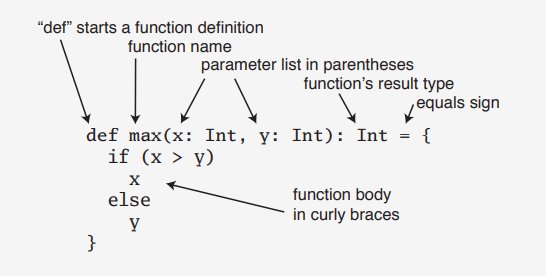
\includegraphics[width=11cm]{func.png} \\
    	Fonte: \cite{Odersky}
    \end{figure}

	No exemplo acima existe uma função chamada max que retorna um valor int, ainda possui dois parâmetros: x e y, ambos com tipagem int. Nessa função, o retorno será decidido por alguma operação dentro das chaves, nesse caso um if, que escolhe entre x e y.
	
	Uma vez criada a função basta chama-la no código principal, para isso é necessário escrever o seu nome e os parâmetros desejados: 
	
	Neste caso:
	\begin{lstlisting}
		max(5, 7)
		
		[Running] 7
	\end{lstlisting}

	Vale lembrar que todo o código Scala é rodado dentro de uma função denominada main, o mesmo ocorre em outras linguagens como C por exemplo. A estrutura do main é dada da seguinte forma:
	
	\begin{lstlisting}[breaklines]
		object hello {
			def main(args: Array[String]): Unit = {
				println("Hello, world!")	
		}	
	}
	\end{lstlisting}
	
	Para realizar um hello world em Scala é necessário primeiro declarar uma classe, para isso se utiliza a expressão "object [nome da classe]", dessa forma podemos criar a função denominada main, onde será rodado o código em Scala. Usaremos como parâmetro o args que é um array de strings, dessa forma será passado uma série de argumentos de linhas de comandos para o código. Além disso é utlizado o tipo de dado Unit como saída, indicando uma saída vázia. Após isso basta utilizar o println como já visto antes.

		\section{Classes}
	
	Segundo \cite{Sfregola2021} classes são estruturas fundamentais para linguagens orientadas a objetos, uma vez que elas são utilizadas para definir um objeto. Elas são extremamente usadas para encapsular dados e alguns comportamentos relacionados entre si.
	
	Para definir uma classe basta usar a palavra-chave 'class' seguida de seu nome.
	Exemplo:
	
	\begin{lstlisting}[breaklines]
	class individuo(nome: String, idade: Int) {
		def saudacao(): Unit = {
			println(s"Ola, meu nome e $nome e eu tenho $idade anos.")
		}
			
		def despedida(nome2: String): Unit = {
			println(s"Adeus $nome2, foi um prazer te conhecer!")
		}
	}
		
	def main(args: Array[String]) = {
		val julio = new individuo("Julio" , 15)
			
		julio.saudacao()
		julio.despedida("Gabriel")
	}
		
	[Running]
	Ola, meu nome e Julio e eu tenho 15 anos.
	Adeus Gabriel, foi um prazer te conhecer!
	\end{lstlisting}

	Note que no exemplo dado inicialmente foi criada a classe "individuo" junto de suas entradas, nesse caso o nome e a idade do individuo. Após isso, foram criadas algumas funções, nesse caso chamadas de métodos, sendo esses o método saudacao, que ira realizar um print com o nome e idade, e o outro método sendo o despedida, que irá receber uma entrada, sendo essa um novo nome que será printada no código. Já no main é realizado a declaração da classe e suas respectivas chamadas.

   %%%%%%%%======================
    \section{Listas}
    %%%%%%%%======================

	Segundo \cite{Sfregola2021} em Scala, listas são uma reunião de elementos/dados que são imutáveis de um mesmo tipo. Ou seja, uma vez criada uma lista, não é possível altera-la, porém todos os métodos possíveis de adicionar ou remover elementos de uma lista retornam uma nova lista com as alterações efetuadas.
	
	Para criar uma lista, é necessário utilizar a classe list ou uma sintaxe construtora de listas.
	
	Exemplo de uma lista com 3 elementos:
	
	\begin{lstlisting}
	def main(args: Array[String]) = {
		val lista1 = List(1, 2, 3)
	
		val lista2 = 4 :: 5 :: 6 :: Nil
	
		val lista3 : List [Int] = List (7, 8, 9)
	
		println(lista1)
	
		println(lista2)
	
		println(lista3)
	}

	[Running] 
	List(1, 2, 3)
	List(4, 5, 6)
	List(7, 8, 9)
	\end{lstlisting}
	
	Note que na primeira linha foi necessário utilizar a classe "List" com o objetivo de criar a lista com os 3 números inteiros solicitados. Já na segunda foi utilizada uma sintaxe construtora de lista, sendo que nela o operador "::" adiciona elementos a lista e o operador "Nil" é usado para representar uma lista vazia. E por último na terceira linha também é usada a classe "List", porém nesse caso é identificado o tipo dos valores da lista.
	
	Ainda é possível mostrar como saída os valores da lista por índice, para isso basta identificar a posição que deseja mostrar para o usuário. Vale lembrar que a contagem dos índices sempre começa pelo valor 0.
	
	Exemplo:
	\begin{lstlisting}
		def main(args: Array[String]) = {
			val lista1 = List(1, 2, 3)
			
			println(lista1(0))
			println(lista1(1))
			println(lista1(2))
		}
	
		[Running] 
		1
		2
		3
	\end{lstlisting}

	\subsection{Operações}
	
	Em Scala é muito comum o uso das operações com listas, visto a sua alta capacidade de utilização, permitindo o programador efetuar uma série de manipulações diferentes de maneira simples e extremamente eficiente.
	
	Considerando as listas: lista1 = (1,2,3) e a lista2 = (4, 5, 6), veja alguns exemplos de operações com essas listas:
	
	\begin{lstlisting}[breaklines]
		// concatenacao
		val lista3 = lista1 ++ lista2
		[Running] List(1, 2, 3, 4, 5, 6)
		
		// adicionando elementos
		val lista4 = lista1 :+ 4 
		[Running] List(1, 2, 3, 4)
		
		// removendo elementos
  		val lista5 = lista1.filterNot(_ == 3) //remove o elemnto 3
  		[Running] List(1, 2)
  		
  		// mapeamento
  		val lista6 = lista1.map(_ * 2) //multiplica a lista por 2
  		[Running] List(2, 4, 6)
  		
  		// reduzindo elementos
  		val red = lista2.reduce(_ + _) //soma todos os elementos
  		[Running] 15
	\end{lstlisting}

    %%%%%%%%======================
    \section{Tuplas}
    %%%%%%%%======================

	Segundo \cite{Odersky}: "Assim como as listas, as tuplas são imutáveis, mas ao contrário das listas, as tuplas podem conter diferentes tipos de elementos". Ou seja, não é possível alteras os valores de uma tupla, porém diferente das listas, uma mesma tupla pode conter um dado do tipo inteiro e outro dado do tipo string por exemplo.
	
	Para criar uma tupla em Scala é necessário inicia-la usando parênteses separando os seus elementos por vírgula.
	
	Exemplo de uma tupla composta por uma string e um float:
	
	\begin{lstlisting}
		def main(args: Array[String]) = {
			val tupla1 = ("Ola!", 3.14)
			
			println(tupla1)
		}
	
		[Running] (Ola!,3.14)
	\end{lstlisting}

	Os elementos do interior de uma tupla podem ser acessados por meio da notação "NomeDaTupla.\_Posição", sendo que a posição diferente de uma lista começa pelo número 1.
	
	\begin{lstlisting}
		def main(args: Array[String]) = {
			val tupla1 = ("Ola!", 3.14)
			
			println(tupla1._1)
			println(tupla1._2)
		}
	
		[Running]
		Ola!
		3.14
	\end{lstlisting}

	\subsection{Operações}
	Assim como as listas, as tuplas apresentam algumas operações possíveis que podem ser extremamente uteis durante a programação. Considerando a tupla val tupla1 = ("Ola!", 3.14), veja alguns exemplos das operações mais comuns envolvendo tuplas em Scala.
	
	\begin{lstlisting}[breaklines]
		//Desestruturar tupla
		val (msg, pi) = minhaTupla //atribui o valor da tupla a variaveis individuais
		
		println(msg)
		println(pi)
		
		[Running] 
		Ola!
		3.14
		
		//Concatenar tuplas
		val tupla2 = ("x", 2)
		val tupla3 = tupla1 ++ tupla2
		println(tupla3)
		
		[Running] (Ola!,3.14,x,2)
		
		//Verificar Tamanho
		val range = tupla1.size
		println(range)
		
		[Running] 2
		
		//Transformar tupla em lista
		val tupla1 = ("Ola!", "mundo")
		val lista = tupla1.toList
		println(lista)
		
		[Running] List(Ola!, mundo)
	\end{lstlisting}


   %%%%%%%%======================
    \section{Set}
    %%%%%%%%======================

	De acordo com \cite{Odersky}, em Scala um set é uma estrutura responsável por agrupar um conjunto de elementos porém sem permitir uma "duplicata" dos mesmos, ou seja, cada elementos presente em um set é único e não possui uma cópia de si mesmo. O conteúdo de um set é armazenado em uma ordem não definida e não possui nenhum índice associado a ele.
	
	Para se implementar um set é necessário usar uma estrutura de dados chamada de "hash table". Isso permite que muitas operações como as de adição, remoção e verificação possam ser executadas constantemente, fazendo com que os sets sejam extremamente eficazes na manipulação de big data.
	
	Exemplo:
	
	\begin{lstlisting} [breaklines]
		val materias = Set("fisica", "calculo", "programacao")
		
		println(materias)
		
		[Running] Set(fisica, calculo, programacao)
	\end{lstlisting}

	Em Scala, a estrutura set apresenta 2 tipos, o tipo mutável e o tipo imutável. O primeiro como o próprio nome diz não podem ser mudados depois de criados, ou seja, qualquer operação de adição ou remoção de elementos, por exemplo, feita em um set imutável retorna um novo set para o usuário. Já o set mutável é o oposto, ou seja, são estruturas que podem ser modificadas depois de sua criação, porém para cria-las é necessário utilizar a biblioteca "scala.collection.mutable.Set".
	
	Operações com set imutável: 
	
	\begin{lstlisting}[breaklines]
		//criando set
		val seq = Set(1, 2, 3)
		
		//adicionando elemento 
		val newseq = seq + 4
		
		//removendo elemento
		val remseq = seq - 3
		
		//unindo set
		val newset = Set(4, 5, 6)
		val uniset = seq ++ newset
		
		//verifica a existencia de um elemento
		val existe1 = seq.contains(1)
		
		//verfica o tamanho do set
		val range = seq.size
	\end{lstlisting}

	Operações com set mutável: 
	
	\begin{lstlisting}
		//importando biblioteca
		import scala.collection.mutable.Set
		
		//criando set vazio
		val seq = Set[Int]()
		
		//adicionando elemento
		seq += 7
		seq += 8
		seq += 9
		
		//removendo elemento
		seq -= 9
		
		//atualizando elemento
		seq.update(7, 3) //substitui o 7 pelo 3
		
		//verificando a existencia de um elemento
		seq.contains(8)
		
		//limpando set
		seq.clear()
	\end{lstlisting}

   %%%%%%%%======================
    \section{Map}
    
    Em Scala, "map" é uma coleção de elementos que armazena chaves e valores relacionados. É um conjunto de dados extremamente eficiente para realizar consultas, pesquisas e operações se baseando nas chaves.
    
    Como criar um map em Scala:
    
    \begin{lstlisting}
    	val map = Map("key1" -> 1, "key2" -> 2, "key3" -> 3)
    	
    	println(map("key1"))
    	
    	[Running] 1
    	
    	
    \end{lstlisting}

	Para criar uma estrutura map em Scala, basta utilizar a classe "Map", e indicar as chaves e longo em seguida o valor específico dessa chave.
	
	Algumas operações com map:
	\begin{lstlisting}[breaklines]
		val map = Map("key1" -> 1, "key2" -> 2, "key3" -> 3)
		
		//update: rertorna um novo map com valores atualizados
		map + (key4 -> 4)
		
		//remove: retorna um novo map sem o par da chave
		map - "key1"
		
		//contains: verifica se o map possui uma chave
		map.contains(key2)
		
		//isEmpty: verifica se o map esta vazio
		map.isEmpty
		
		//size: retorna o tamanho do map
		map.size
		
		//keySet: retorna todas as chaves do map
		map.keySet
		
		//values: retorna todos os valores do map
		map.values
	\end{lstlisting}
    %%%%%%%%======================

	\section{Array}
	
	Segundo \cite{Odersky}, em Scala um array é um conjunto de elementos armazenados e uma sequência fixa, e diferente das outras coleções imutáveis como set e lista, é possível alterar os valores presentes em um array mesmo após a sua criação, ou seja, o array é uma estrutura mutável.
	
	Em Scala, todo array apresenta uma estrutura um tamanho fixo determinada determinado na sua criação, sendo que todos os seus elementos devem apresentar o mesmo tipo de dado, ou seja, array é uma estrutura de tipo homogêneo.
	
	Como criar um array:
	\begin{lstlisting}
		val array1: Array[Int] = Array(1,2,3)
		
		println(array1(2))
		
		[Running] 3
	\end{lstlisting}

	Para criar um array basta utilizar a classe e indicar os seus elementos.
	
	Algumas operações:
	\begin{lstlisting}
		//criando array
		val array1: Array[Int] = Array(1,2,3)
		
		//acessa o valor do indice informado
		array1(0)
		
		//modifica elemento no indice informado
		array1 = 6
		
		//tamanho do array
		array1.length
	\end{lstlisting}


% Prof. Dr. Ausberto S. Castro Vera
% UENF - CCT - LCMAT - Curso de Ci\^{e}ncia da Computa\c{c}\~{a}o
% Campos, RJ,  2023
% Disciplina: Paradigmas de Linguagens de Programa\c{c}\~{a}o
% Aluno: Gabriel Costa Fassarella



\chapter{ Aplica\c{c}\~{o}es da Linguagem Scala}

Neste capítulo será abordado algumas simples aplicações da linguagem Scala, apresentando o código fonte junto de imagens com sua aplicação e resultados assim como uma breve descrição do código.



    %%%--------------------------------------------------------------------
    \section{Operações Básicas}
    %%%--------------------------------------------------------------------
    O código que será abordado nessa seção se trata de uma simples implementação de uma calculadora do volume de um cilindro em Scala. Esse algoritmo exige ao usuário a entrada dos dados necessários para o cálculo (raio e altura) por meio de um menu interativo, e retorna ao mesmo o valor da área do cilindro.
    
    Código fonte:
    \begin{lstlisting}[breaklines]
import scala.io.StdIn

object CalculadoraCilindro {
	def main(args: Array[String]): Unit = { // Definindo o main, local em que o codigo sera rodado
		var continuar = true // Condicao de existencia do while
		
		while (continuar) {
			println("1. Calcular volume do cilindro") // Menu
			println("2. Sair")
			val op = StdIn.readInt() // Dando entrada na opcao
			
			op match {
				case 1 => // Entrada dos dados do cilindro
				println("Digite o raio do cilindro:")
				val raio = StdIn.readDouble()
				println("Digite a altura do cilindro:")
				val altura = StdIn.readDouble()
				val volume = calcVol(raio, altura)
				println(s"O volume do cilindro e: $volume")
				
				case 2 => // Fim do codigo
				continuar = false
				println("Encerrando o programa.")
				
				case _ => // Erro na entrada
				println("Opcao invalida. Por favor, tente novamente.")
			}
			println()
		}
	}
	
	def calcVol(raio: Double, altura: Double): Double = { // Calculo do volume
		val areaB = 3.14 * raio * raio
		val volume = areaB * altura
		volume // Retorna o volume
	}
}
    \end{lstlisting}

	\begin{itemize}
		
		\item Inicialmente é importada a biblioteca responsável pela entrada de dados.
		
		\item Em seguida é criado o main, área principal no qual o código é rodado.
		
		\item Após isso é mostrado o menu ao usuário, exigindo ao mesmo uma entrada. Vale lembrar que esse menu é criado dentro de um while, para caso o usuário deseje calcular a área de mais de um cilindro.
		
		\item Após isso é criada uma estrutura match para os casos apresentados na leitura do menu. A primeira opção ocorre caso op seja 1, com isso são dadas as entradas do cilindro. A segunda opção é para caso op seja 2, quebrando assim o while e finalizando o código. E por último, é casa op seja qualquer outro valor, mostrando assim o menu novamente para o usuário.
		
		\item Com isso, caso op seja 1, será chamada a função de calculo de volume, que recebe o raio e a altura, podendo assim calcular e retornar o valor do volume, e em seguida o mostrando ao usuário. 
		
	\end{itemize}

	Para a implementação desse algoritmo foi utilizada a Ide Vscode, para isso foi criado um projeto e escrito o código. Veja as imagens da implementação do programa e dos resultados obtidos ao compilar:
	
	\begin{figure}[H]
		\centering
		\caption{Implementação Operações}
		\label{Implementação Operações}
		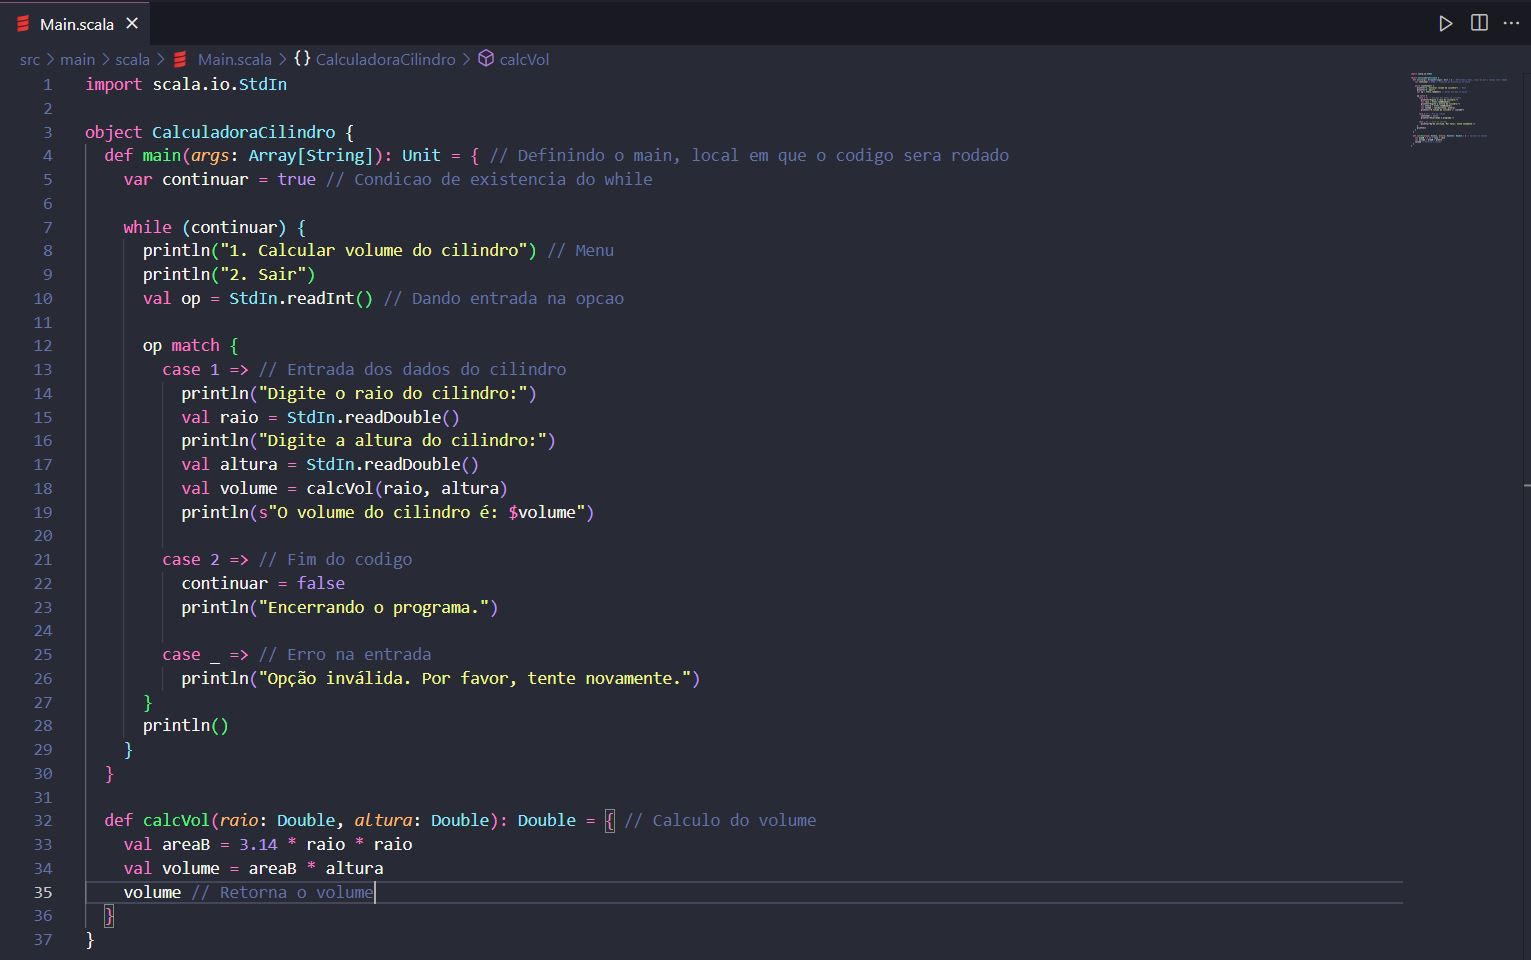
\includegraphics[width=17cm]{Pictures/Operac.jpg} \\
		Fonte: Autor do Livro
	\end{figure}

	Resultados ao compilar o arquivo:
	
	\begin{figure}[H]
		\centering
		\caption{Resultados Implementação Operações}
		\label{Resultados Implementação Operações}
		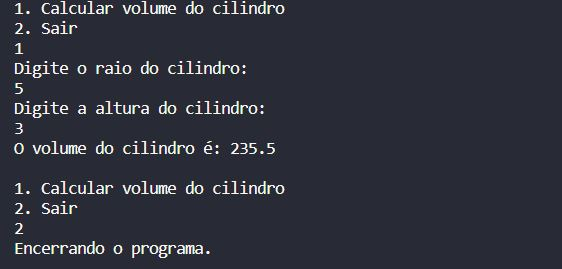
\includegraphics[width=8cm]{Pictures/ResOperac.jpg} \\
		Fonte: Autor do Livro
	\end{figure}


    %%%--------------------------------------------------------------------
    \section{Calculadora}
    %%%--------------------------------------------------------------------
    
   	O algoritmo a ser apresentado nesta seção é um exemplo simples de uma calculadora que é capaz de realizar as 4 operações matemáticas básicas: adição, subtração, multiplicação e divisão. O objetivo desse algoritmo é dar a possibilidade ao usuário de realizar as 4 operações com os números fornecidos.  
    
    Código fonte: 
    \begin{lstlisting}[breaklines]
// Definindo a classe Calculadora
class Calculadora {
	// Definindo as operacoes basicas da classe (metodos)
	def add(a: Int, b: Int): Int = a + b
	
	def sub(a: Int, b: Int): Int = a - b
	
	def mult(a: Int, b: Int): Int = a * b
	
	def div(a: Float, b: Float): Float = {
		if (b != 0) //Verificando se ocorre uma divisao por 0
		a / b
		else
		throw new ArithmeticException("Divisao por zero nao e permitida!")
	}
}

// Definindo o main, onde o programa sera rodado
object Main {
	def main(args: Array[String]): Unit = {
		// Criando uma instancia da classe Calculadora
		val calculadora = new Calculadora()
		
		// Realizando as operacoes
		val sum = calculadora.add(4, 2)
		val dif = calculadora.sub(4, 2)
		val prod = calculadora.mult(4, 2)
		val quot = calculadora.div(4, 2)
		
		// Imprimindo os resultados
		println(s"Soma: $sum")
		println(s"Diferenca: $dif")
		println(s"Produto: $prod")
		println(s"Quociente: $quot")
	}
}
    \end{lstlisting}
	\begin{itemize}
		\item Inicialmente, é definida uma classe chamada "calculadora", com seus 4 métodos que representam as 4 operações básicas.
		
		\item O método "add" recebe 2 valores inteiros e os soma, o método "sub" recebe 2 inteiros e os subtrai, o método "mult" recebe 2 inteiros e os multiplica, e por último o método "div" recebe 2 floats, verifica se o segundo é diferente de 0 (para evitar uma indefinição) e caso não seja será realizada a divisão de a por b.
		
		\item Em seguida é criado o main, local que será o ponto de partida do programa.
		
		\item No interior do main é criada uma nova instância da classe calculadora.
		
		\item Por meio dessa instância criada, são realizadas as operações matemáticas desejadas, armazenando os resultados em variáveis.
		
		\item E por último são mostrados os valores para o usuário.
	\end{itemize}

	A implementação desse código fonte em uma Ide é extremamente simples, basta criar um projeto e escrever o código em na Ide desejada. Neste caso, foi utilizado como Ide o Vscode, veja o exemplo abaixo:
	
	\begin{figure}[H]
		\centering
		\caption{Implementação Calculadora}
		\label{Implementação Calculadora}
		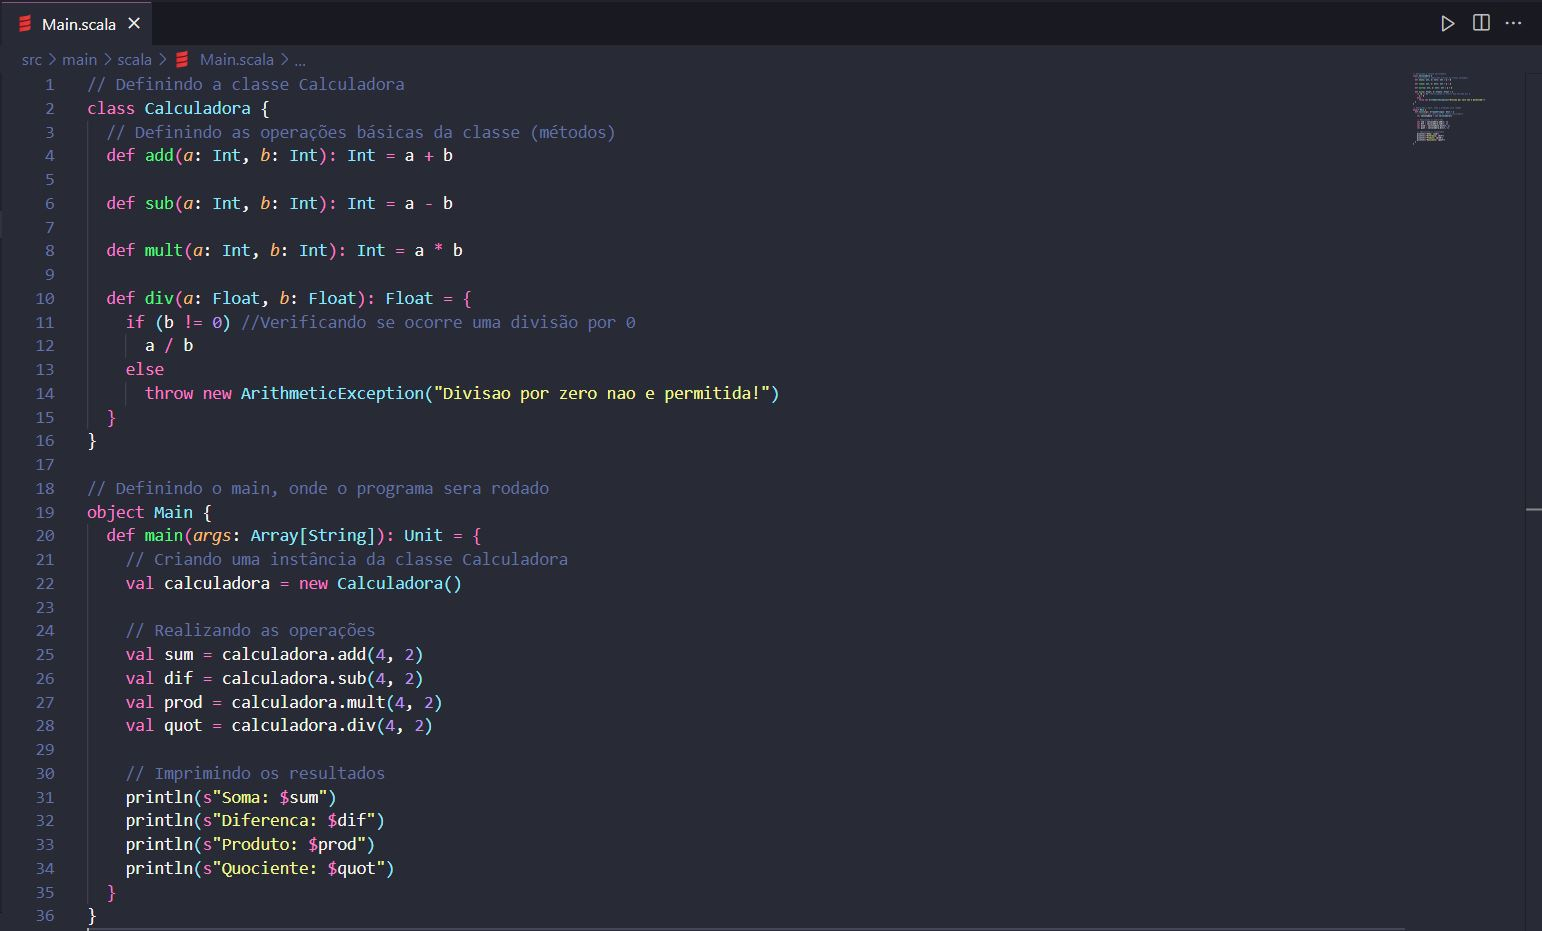
\includegraphics[width=17cm]{Pictures/Calc.jpg} \\
		Fonte: Autor do Livro
	\end{figure}

	Resultados obtidos ao compilar o algoritmo: 
	
	\begin{figure}[H]
		\centering
		\caption{Resultados Implementação Calculadora}
		\label{Resultados Implementação Calculadora}
		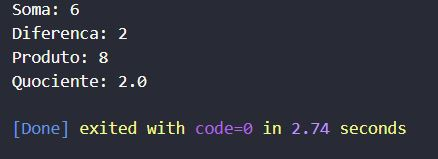
\includegraphics[width=8cm]{Pictures/ResCalc.jpg} \\
		Fonte: Autor do Livro
	\end{figure}
    %%%--------------------------------------------------------------------
    
    \section{Regra do Trapézio}
    Nessa seção será apresentada uma aplicação de um código em Scala responsável por calcular o valor aproximado de uma integral definida em um intervalo de a até b. Para isso será utilizado um conceito do cálculo numérico denominado Regra do Trapézio Generalizado.
    
    Código fonte:
    
    \begin{lstlisting}[breaklines]
object RegraDoTrapezio {
	def main(args: Array[String]): Unit = {
		val a = 0.0 // Limite inferior do intervalo
		val b = 2.0 // Limite superior do intervalo
		val n = 10 // Numero de subintervalos
		
		val h = (b - a) / n // Tamanho de cada subintervalo
		val x = Array.tabulate(n + 1)(i => a + i * h) // Pontos xi tal que i = 0, 1, ..., n
		val y = x.map(f) // Valores de f(xi) para cada xi
		
		val integral = (h / 2) * (y.head + 2 * y.drop(1).dropRight(1).sum + y.last)
		
		println(s"Aproximacao da integral: $integral")
	}
	
	def f(x: Double): Double = {
		// Definindo a funcao que sera integrada
		x * x // f(x) = x^2
	}
}
    \end{lstlisting} 

	\begin{itemize}
		\item Inicialmente no main é definido os limites inferiores e superiores da integral, assim o número de subintervalos que serão utilizados para o calculo.
		
		\item Com isso será calculado o valor de h, que será o passo entre os pontos de amostragem.
		
		\item Após calcular o h (o passo), será efetuado do valor de todos os xi relacionados a cada subintervalo, assim como o f(xi) associado a cada subintervalo.
		
		\item Com isso será calculado o valor aproximado da integral, para isso basta aplicar a formula da regra do trapézio generalizado:
		\[
		\text{{Integral}} \approx \frac{h}{2} \left( y_0 + 2 \sum_{i=1}^{n-1} y_i + y_n \right)
		\]
		onde:
		\begin{align*}
			h & : \text{{tamanho do subintervalo}} \\
			y_0, y_1, ..., y_n & : \text{{valores da função nos pontos de amostragem}}
		\end{align*}
	\end{itemize}
    
    Com isso já é possível implementar esse código em um ambiente de programação adequado. Para isso foi escolhido a Ide Vscode, veja abaixo a implementação do algoritmo e o valor obtido com sua compilação.
    
    Implementação:
    
	\begin{figure}[H]
		\centering
		\caption{Implementação Regra do Trapézio Generalizado}
		\label{Implementação Regra do Trapézio Generalizado}
		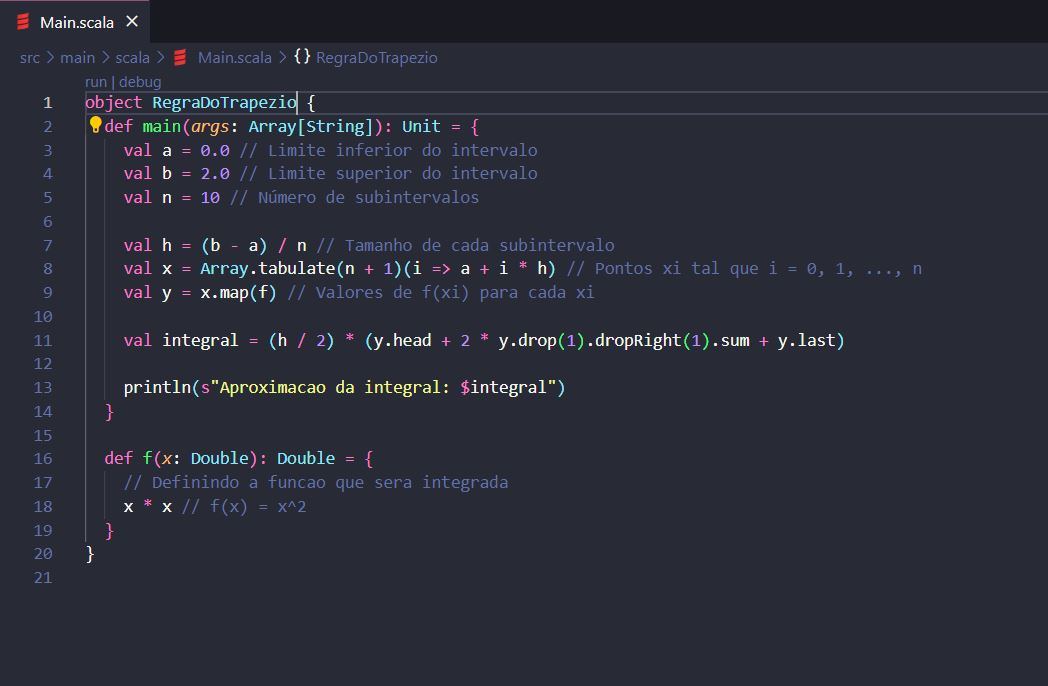
\includegraphics[width=17cm]{Pictures/Integral.jpg} \\
		Fonte: Autor do Livro
	\end{figure}
    
    Resultado obtido ao compilar o algoritmo: 
    
    \begin{figure}[H]
    	\centering
    	\caption{Resultados Implementação Regra do Trapézio Generalizado}
    	\label{Resultados Implementação Regra do Trapézio Generalizado}
    	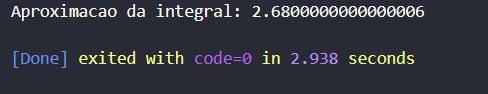
\includegraphics[width=8cm]{Pictures/ResIntegral.jpg} \\
    	Fonte: Autor do Livro
    \end{figure}
    
    \section{Bubble Sort}
    %%%--------------------------------------------------------------------
    O bubble sort é um clássico algoritmo de ordenação de dados muito utilizado para organizar valores de um vetor. O algoritmo funciona percorrendo todos os elementos de uma lista, comparando os valores adjacentes e caso estejam na ordem errada é realizada uma troca. Isso ocorre até o array estar completamente ordenado.
      
    Código fonte:
    \begin{lstlisting}[breaklines]
object BubbleSortExample {
	def BubbleSort(arr: Array[Int]): Array[Int] = { // Funcao de bubble sort
		val n = arr.length // Definindo o tamanho do array
		for (i <- 0 until n - 1) { // For para percorrer o array
			for (j <- 0 until n - i - 1) { // For para percorrer o array e realizar as comparacoes
				if (arr(j) > arr(j + 1)) { // Verificando se o proximo valor e menor que o valor atual
					val temp = arr(j) // Troca
					arr(j) = arr(j + 1)
					arr(j + 1) = temp
				}
			}
		}
		arr // Retorna
	}
	
	def main(args: Array[String]): Unit = { // Definindo o main
		val array = Array(64, 34, 25, 12, 22, 11, 90) // Definindo o array
		val sortArray = BubbleSort(array) // Chamada da funcao
		println(sortArray.mkString(", ")) // Mostrando para o usuario
	}
}
    \end{lstlisting}

	\begin{itemize}
		\item Inicialmente no main, é definido um array com elementos aleatórios de maneira desordenada.
		
		\item Em seguida é realizada a chamada da função bubble sort.
		
		\item Logo em seguida, o tamanho do array é salvo na variável.
		
		\item Em seguida é criado um for externo responsável por percorrer o array.
		
		\item Também é criado um for interno, responsável por percorrer o array e realizar as comparações entre o elemento na posição j e seu sucessor, caso o valor na posição j seja maior que na posição j + 1, ocorre uma troca.
		
		\item Com o fim de ambos os loops, o array organizado é retornado e mostrado ao usuário.
	\end{itemize}

	A implementação desse algoritmo, assim como as anteriores, foi feita criando um projeto na Ide Vscode, veja abaixo a implementação e o resultado obtido com a compilação do arquivo.
	
	Implementação:

	\begin{figure}[H]
		\centering
		\caption{Implementação Bubble Sort}
		\label{Implementação Bubble Sort}
		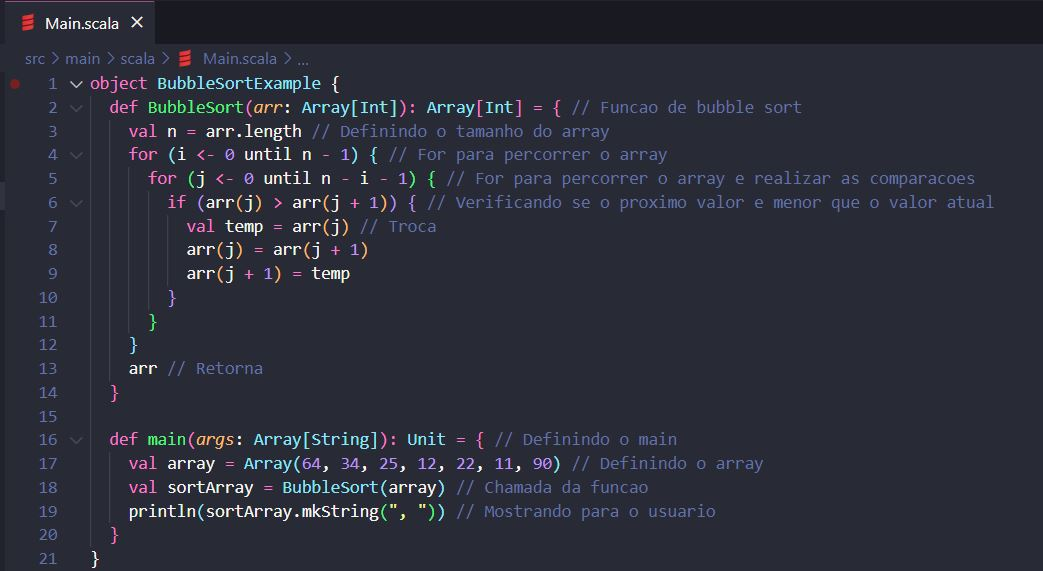
\includegraphics[width=17cm]{Pictures/bubble.jpg} \\
		Fonte: \href{https://www.includehelp.com/scala/implement-an-arithmetic-calculator-using-a-match-case.aspx}{Clique Aqui}
	\end{figure}

	Resultados obtidos quando o arquivo é compilado:

	\begin{figure}[H]
		\centering
		\caption{Resultados Implementação Bubble Sort}
		\label{Resultados Implementação Bubble Sort}
		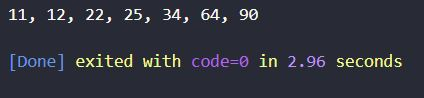
\includegraphics[width=8cm]{Pictures/resBubble.jpg} \\
		Fonte: \href{https://www.includehelp.com/scala/implement-an-arithmetic-calculator-using-a-match-case.aspx}{Clique Aqui}
	\end{figure}

    %%%--------------------------------------------------------------------
    \section{Quick Sort}
    %%%--------------------------------------------------------------------
    O quick sort é um clássico e extremamente efetivo algoritmo de ordenação, por isso recebe o nome de quick sort. Ele funciona selecionando um elemento do array que será chamado de pivô, com isso é seguido a lógica de separar o vetor em 2, uma parte com valores menores que o pivô e outra parte com valores maiores que o pivô, buscando assim coloca-lo em sua respectiva posição.
    
    Código fonte:
    
    \begin{lstlisting}[breaklines]
object QuickSort {
	def main(args: Array[String]): Unit = { // Main
		val arr = Array(64, 34, 25, 12, 22, 11, 90) // Definindo array
		println("Array antes da ordenacao:")
		println(arr.mkString(", "))
		
		quickSort(arr, 0, arr.length - 1) // Chamada da funcao
		
		println("Array apos a ordenacao:")
		println(arr.mkString(", "))
	}
	
	def quickSort(arr: Array[Int], a: Int, b: Int): Unit = { // Definindo funcao quick sort
		if (a < b) { // Caso ainda tenham dados no array
			val pivo = partition(arr, a, b)
			
			// Chamadas recursivas
			quickSort(arr, a, pivo - 1)
			quickSort(arr, pivo + 1, b)
		}
	}
	
	def partition(arr: Array[Int], a: Int, b: Int): Int = {
		val pivo = arr(b) // Define o pivo
		var i = a - 1 
		
		for (j <- a until b) { // Loop para percorrer o array
			if (arr(j) <= pivo) { // Procurando menor valor
				i += 1
				swap(arr, i, j) // Funcao de troca
			}
		}
		
		swap(arr, i + 1, b) // Funcao de troca
		i + 1
	}
	
	def swap(arr: Array[Int], i: Int, j: Int): Unit = { // Funcao de troca
		val temp = arr(i)
		arr(i) = arr(j)
		arr(j) = temp
	}
}
    \end{lstlisting}

	\begin{itemize}
		\item Inicialmente é criado o main e dentro dele é também criado o array com valores aleatórios de maneira desordenada, em seguida é realizada a chamada da função, passando como parâmetros o próprio array, o início e o fim.
		
		\item Após isso é verificado se ainda existem elementos no vetor, se verdadeiro é chamada a função que repartira o array e selecionará o pivô.
		
		\item Dentro dessa função é definido o pivô como o último elemento do array, dentro do loop é verificado se o elemento for menor ou igual ao pivô, incrementamos i e trocamos o elemento na posição i com o elemento na posição j.
		
		\item Após o loop, o último elemento menor ou igual ao pivô está na posição i + 1. Portanto, trocamos o pivô de posição com esse elemento para colocá-lo em sua posição final.
		
		\item Com o fim do loop é retornado a posição do pivô, com isso são feitas as chamadas recursivas dividindo novamente o array, sendo a primeira chamada feita para organizar a esquerda a lista, e a segunda para ordenar a direita do array.
	\end{itemize}

	A implementação desse algoritmo, assim como as anteriores, foi feita criando um projeto na Ide Vscode, veja abaixo a implementação e o resultado obtido com a compilação do arquivo.
	
	Implementação:
	
	\begin{figure}[H]
		\centering
		\caption{Implementação Quick Sort Parte 1}
		\label{Implementação Quick Sort Parte 1}
		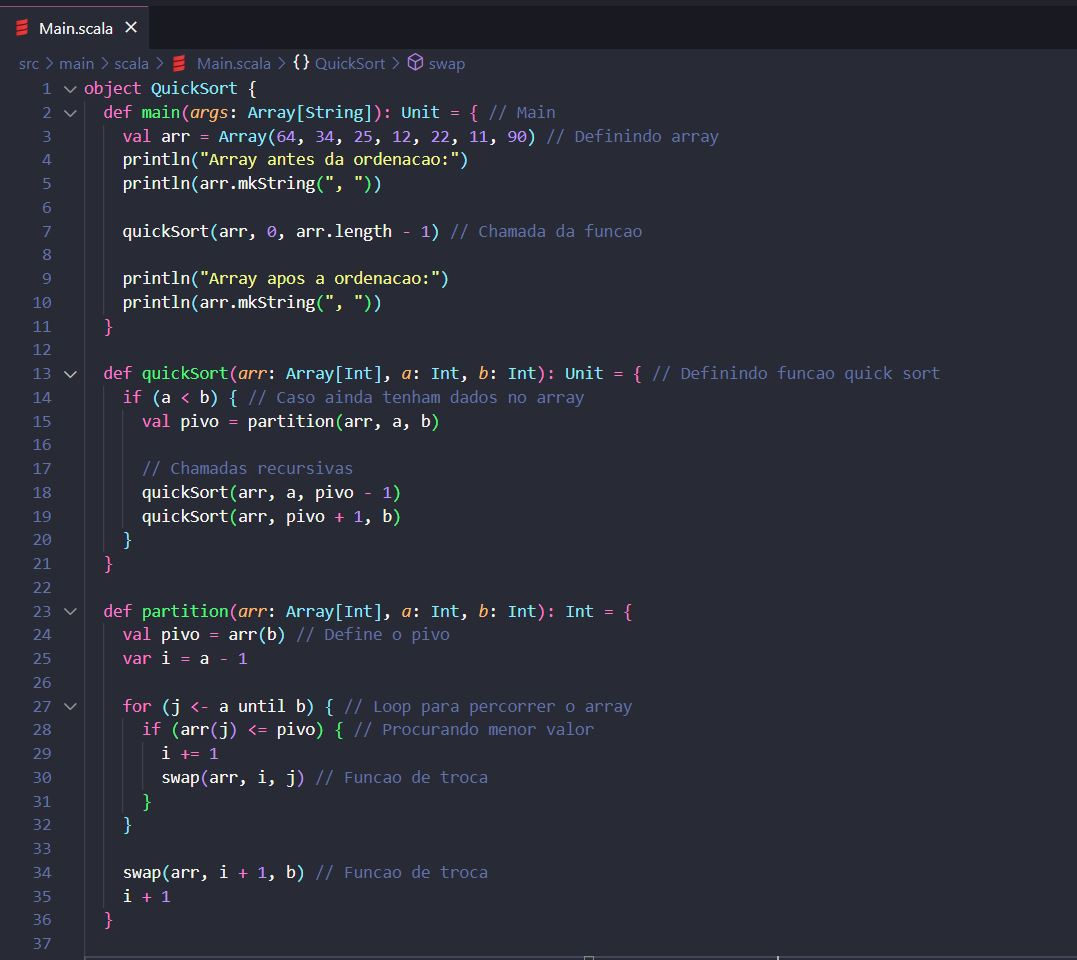
\includegraphics[width=17cm]{Pictures/Quick1.jpg} \\
		Fonte: \href{https://stackoverflow.com/questions/67182087/scala-quicksort-algorithm-implementationi}{Clique Aqui!}
	\end{figure}

	 \begin{figure}[H]
	 	\centering
	 	\caption{Implementação Quick Sort Parte 2}
	 	\label{Implementação Quick Sort Parte 2}
	 	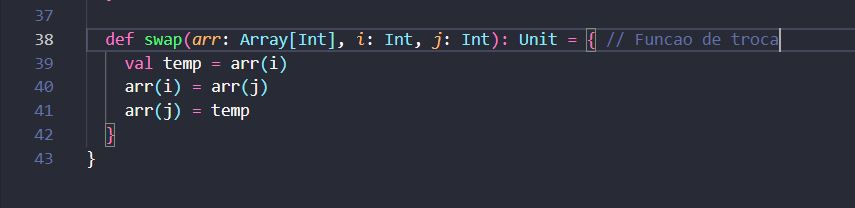
\includegraphics[width=12cm]{Pictures/Quick2.jpg} \\
	 	Fonte: \href{https://stackoverflow.com/questions/67182087/scala-quicksort-algorithm-implementationi}{Clique Aqui!}
	 \end{figure}
 
 	Resultados obtidos ao compilar:
 
 	\begin{figure}[H]
	 	\centering
	 	\caption{Resultados Implementação Quick Sort}
	 	\label{Resultados Implementação Quick Sort}
	 	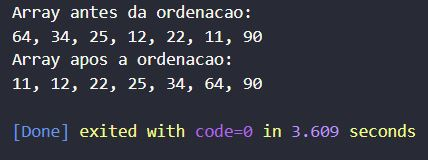
\includegraphics[width=8cm]{Pictures/resQuick.jpg} \\
	 	Fonte: \href{https://stackoverflow.com/questions/67182087/scala-quicksort-algorithm-implementationi}{Clique Aqui!}
 	\end{figure}
 	
 	\section{Equação do Segundo Grau}
 	
 	Essa seção abordará um algoritmo básico de cálculo de uma equação do segundo grau utilizando a conhecida fórmula de bhaskhara. O objetivo desse algoritmo é encontrar as raízes de uma equação do segundo grau fornecida ao programa.
 	
 	\begin{lstlisting}[breaklines]
import scala.math.sqrt // Biblioteca para calculo de raiz

object EquacaoSegundoGrau {
	def CalcEq(a: Double, b: Double, c: Double): Unit = { 
		val delta = b * b - 4 * a * c // Calculo delta
		
		if (delta > 0) { // Existem 2 raizes reais
			val x1 = (-b + sqrt(delta)) / (2 * a) // Calculo raiz 1
			val x2 = (-b - sqrt(delta)) / (2 * a) // Calculo raiz 2
			println("Raizes:")
			println(s"x1 = $x1")
			println(s"x2 = $x2")
		} else if (delta == 0) { // Existe 1 raiz
			val x = -b / (2 * a) // Calculo da raiz
			println("Raiz:")
			println(s"x = $x")
		} else {
			println("A equacao nao possui raizes reais.") // Delta < 0, logo raiz imaginaria
		}
	}
	
	def main(args: Array[String]): Unit = { // Main
		// Coeficientes equacao
		val a = 1.0
		val b = -3.0
		val c = 2.0
		
		CalcEq(a, b, c) // Chamada funcao
	}
}
 	\end{lstlisting}  
 
 	\begin{itemize}
 		\item Inicialmente é dado o import na biblioteca responsável por calcular o valor da raiz quadrada.
 		
 		\item no main é dada a entrada dos coeficientes da equação do segundo grau.
 		
 		\item Na função chamada, é calculado inicialmente o delta, em seguida é verificado se o mesmo é maior que 0, se sim existem 2 raízes que serão calculada e retornadas, se for zero existe apenas uma raiz, e se for menor que 0 ocorrerá uma raiz quadrada de número negativo, logo uma raiz imaginária.
 		
 		\item Em seguida o valor é mostrado ao usuário.
 	\end{itemize}
 
 	A implementação desse código fonte em uma Ide é extremamente simples, basta criar um projeto e escrever o código em na Ide desejada. Neste caso, foi utilizado como Ide o Vscode, veja o exemplo abaixo:
 	
 	Implementação:
 	
 	\begin{figure}[H]
 		\centering
 		\caption{Implementação Equação 2 Grau}
 		\label{Implementação Equação 2 Grau}
 		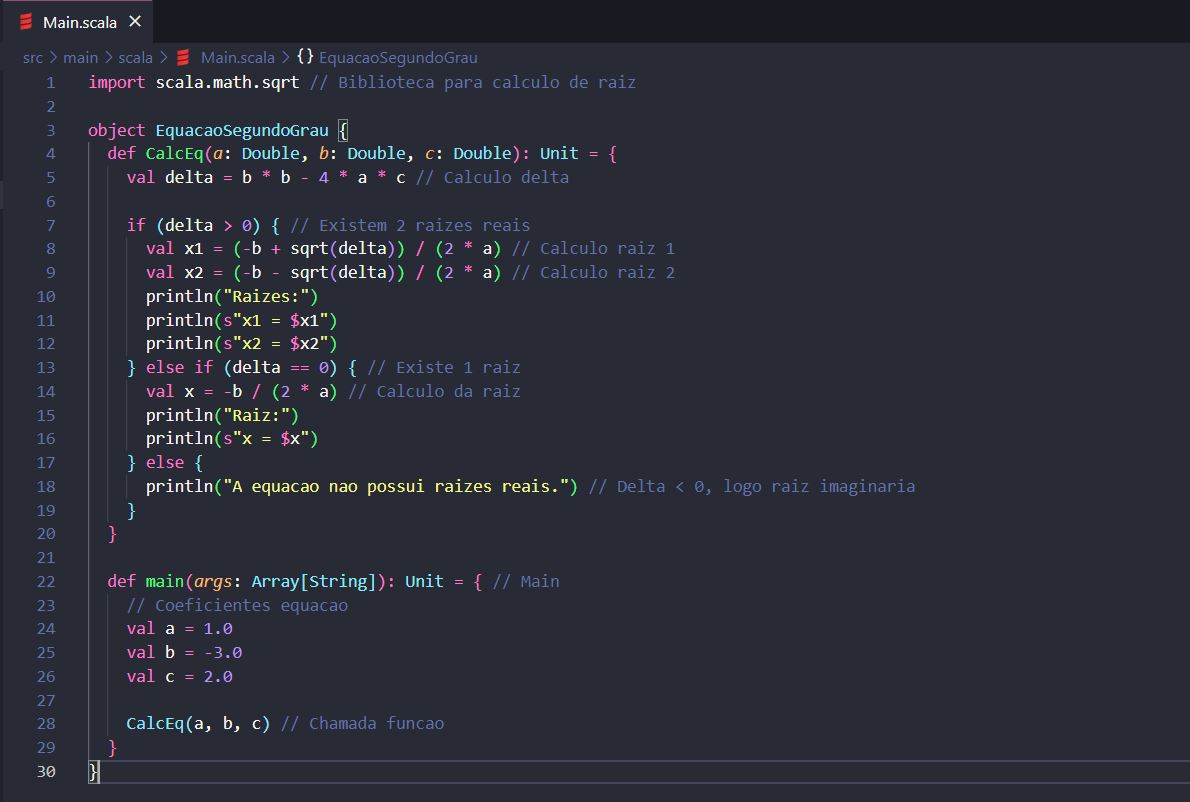
\includegraphics[width=17cm]{Pictures/Eq2Grau.jpg} \\
 		Fonte: Autor do Livro
 	\end{figure}
 	
 	Resultados da compilação:
 	
 	\begin{figure}[H]
		\centering
		\caption{Resultados Equação do 2 Grau}
		\label{Resultados Equação do 2 Grau}
		\includegraphics[width=8cm]{Pictures/resEq2Grau.jpg} \\
		Fonte: Autor do Livro
	\end{figure}


	\section{Sistema Linear}
	
	Nesta seção abordaremos um algoritmo capaz de solucionar um sistema de equações 2x2. Para isso é necessário calcular o determinante da matriz com o objetivo de verificar se existe solução, e caso esse determinante seja diferente de 0, será efetuada a regra de cramer para calcular a solução do sistema.
	
	Código fonte: 
	
	\begin{lstlisting}[breaklines]
object SistemaEquacoes {
	
	def resSist(a11: Double, a12: Double, b1: Double, a21: Double, a22: Double, b2: Double): Option[(Double, Double)] = {
		val det = a11 * a22 - a12 * a21 // Calculo do determinante
		
		if (det != 0) {
			// Calculo solucao
			val x = (b1 * a22 - b2 * a12) / det
			val y = (a11 * b2 - a21 * b1) / det
			Some(x, y)
		} else {
			None // O sistema nao tem solucao unica
		}
	}
	
	def main(args: Array[String]): Unit = {
		// Coeficientes
		val a11 = 2.0
		val a12 = 3.0
		val b1 = 10.0
		val a21 = 1.0
		val a22 = -1.0
		val b2 = -5.0
		
		val solucao = resSist(a11, a12, b1, a21, a22, b2) // Chamada funcao
		
		solucao match {
			case Some((x, y)) =>
			println(s"Solucao: x = $x, y = $y")
			case None =>
			println("O sistema nao tem solucao unica...")
		}
	}
	
}
	\end{lstlisting}

 	\begin{itemize}
 		\item Inicialmente no main é se define o sistema linear desejado no seguinte formato:
 		\begin{lstlisting}
		a11 * x + a12 * y = b1
		a21 * x + a22 * y = b2
 		\end{lstlisting}
 		Com isso é realizada a chamada da função que irá calcular a solução.
 		\item Na função de cálculo de solução é inicialmente calculado o determinante, para verificar se o sistema em questão possui solução ou não, caso o determinante seja diferente de zero é realizada a regra de cramer que dará como resultado a solução do sistema, retornando assim para o usuário. Porém caso o determinante seja igual a 0 será retornado 'none', indicando que o sistema não possui solução única.
 	\end{itemize}
 
 	 Com isso já é possível implementar esse código em um ambiente de programação adequado. Para isso foi escolhido a Ide Vscode, veja abaixo a implementação do algoritmo e o valor obtido com sua compilação.
 	 
 	 Implementação:
 	 
 	 \begin{figure}[H]
 	 	\centering
 	 	\caption{Implementação Sistema Linear}
 	 	\label{Implementação Sistema Linear}
 	 	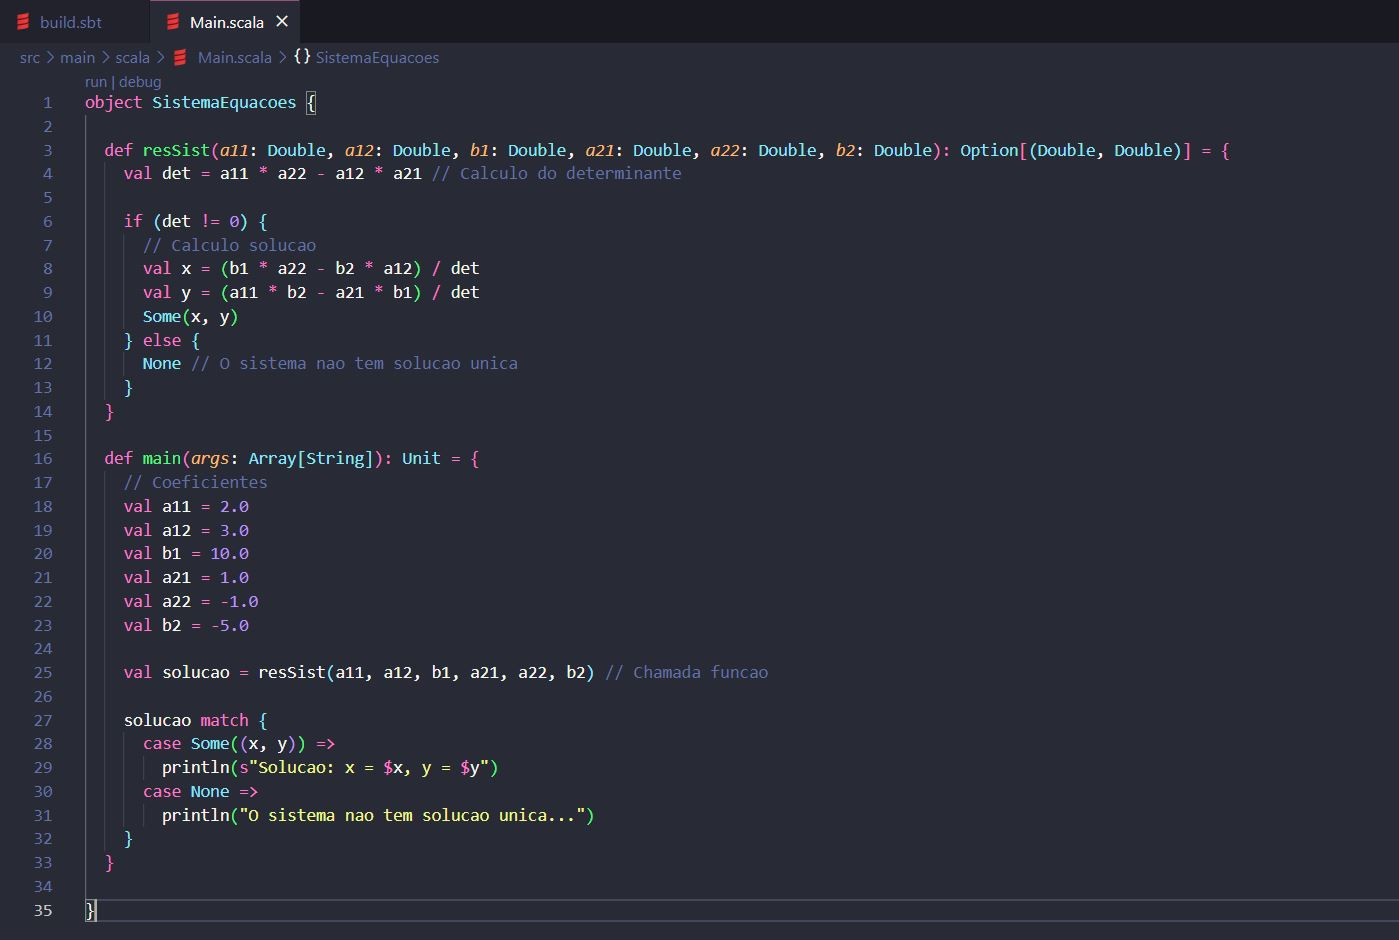
\includegraphics[width=17cm]{Pictures/Sist.jpg} \\
 	 	Fonte: Autor do Livro
 	 \end{figure}
  
  
	 Resultados da compilação:
	  
	\begin{figure}[H]
	 	\centering
	 	\caption{Resultados Sistema Linear}
	 	\label{Resultados Sistema Linear}
	 	\includegraphics[width=8cm]{Pictures/resSist.jpg} \\
	 	Fonte: Autor do Livro
	\end{figure}

% Prof. Dr. Ausberto S. Castro Vera
% UENF - CCT - LCMAT - Curso de Ci\^{e}ncia da Computa\c{c}\~{a}o
% Campos, RJ,  2023
% Disciplina: Paradigmas de Linguagens de Programa\c{c}\~{a}o
% Aluno: Gabriel Costa Fassarella



\chapterimage{ScalaH} % Chapter heading image ==>  Trocar este arquivo por outro 1200x468
\chapter{Ferramentas existentes e utilizadas}

Neste capítulo serão apresentadas duas ferramentas que foram utilizadas no desenvolvimento desse livro, e que também podem ser usadas pelo leitor. São elas: o Visual Studio Code (VS Code) e o Scastie.
\begin{itemize}
  \item Nome da ferramenta (compilador-interpretador)
  \item Endere\c{c}o na Internet
  \item Vers\~{a}o atual e utilizada
  \item Descri\c{c}\~{a}o simples (m\'{a}x 2 par\'{a}grafos)
  \item Telas capturadas da ferramenta
  \item Outras informa\c{c}\~{o}es
\end{itemize}


    \section{Visual Studio Code (VS Code)}
	Segundo \cite{Plainer}, o Visual Studio Code, ou simplesmente VS Code, é uma IDE desenvolvida pela Microsoft. Ela é um ambiente de programação gratuito e de código aberto que possui o suporte para inúmeras linguagens de programação diferentes e que pode ser executada em diversos sistemas operacionais, como o Windows, macOS ou Linux.
	
	Uma das principais características do VS Code é apresentar uma interface gráfica extremamente leve e personalizável, além disso a IDE fornece ao usuário uma diversa quantia de recursos como extensões que podem ser instaladas fornecendo ao usuário uma ampla gama de possibilidades. Isso faz com que a IDE suporte várias linguagens de programação diferentes, e para que a IDE rode códigos em Scala, é necessário duas extensões diferentes, a primeira o Scala Syntax e o Scala Metals, e além disso é necessário compilar os códigos na linguagem, para isso deve-se instalar a extensão Code runner. Vale lembrar que durante o desenvolvimento desse livro, foi utilizada a IDE na versão 1.79.1.
	
	A IDE pode ser instalada em sua atual versão \href{https://code.visualstudio.com}{aqui}.

	Imagens da ferramenta com a implementação de alguns códigos simples:
	
	\begin{figure}[H]
		\centering
		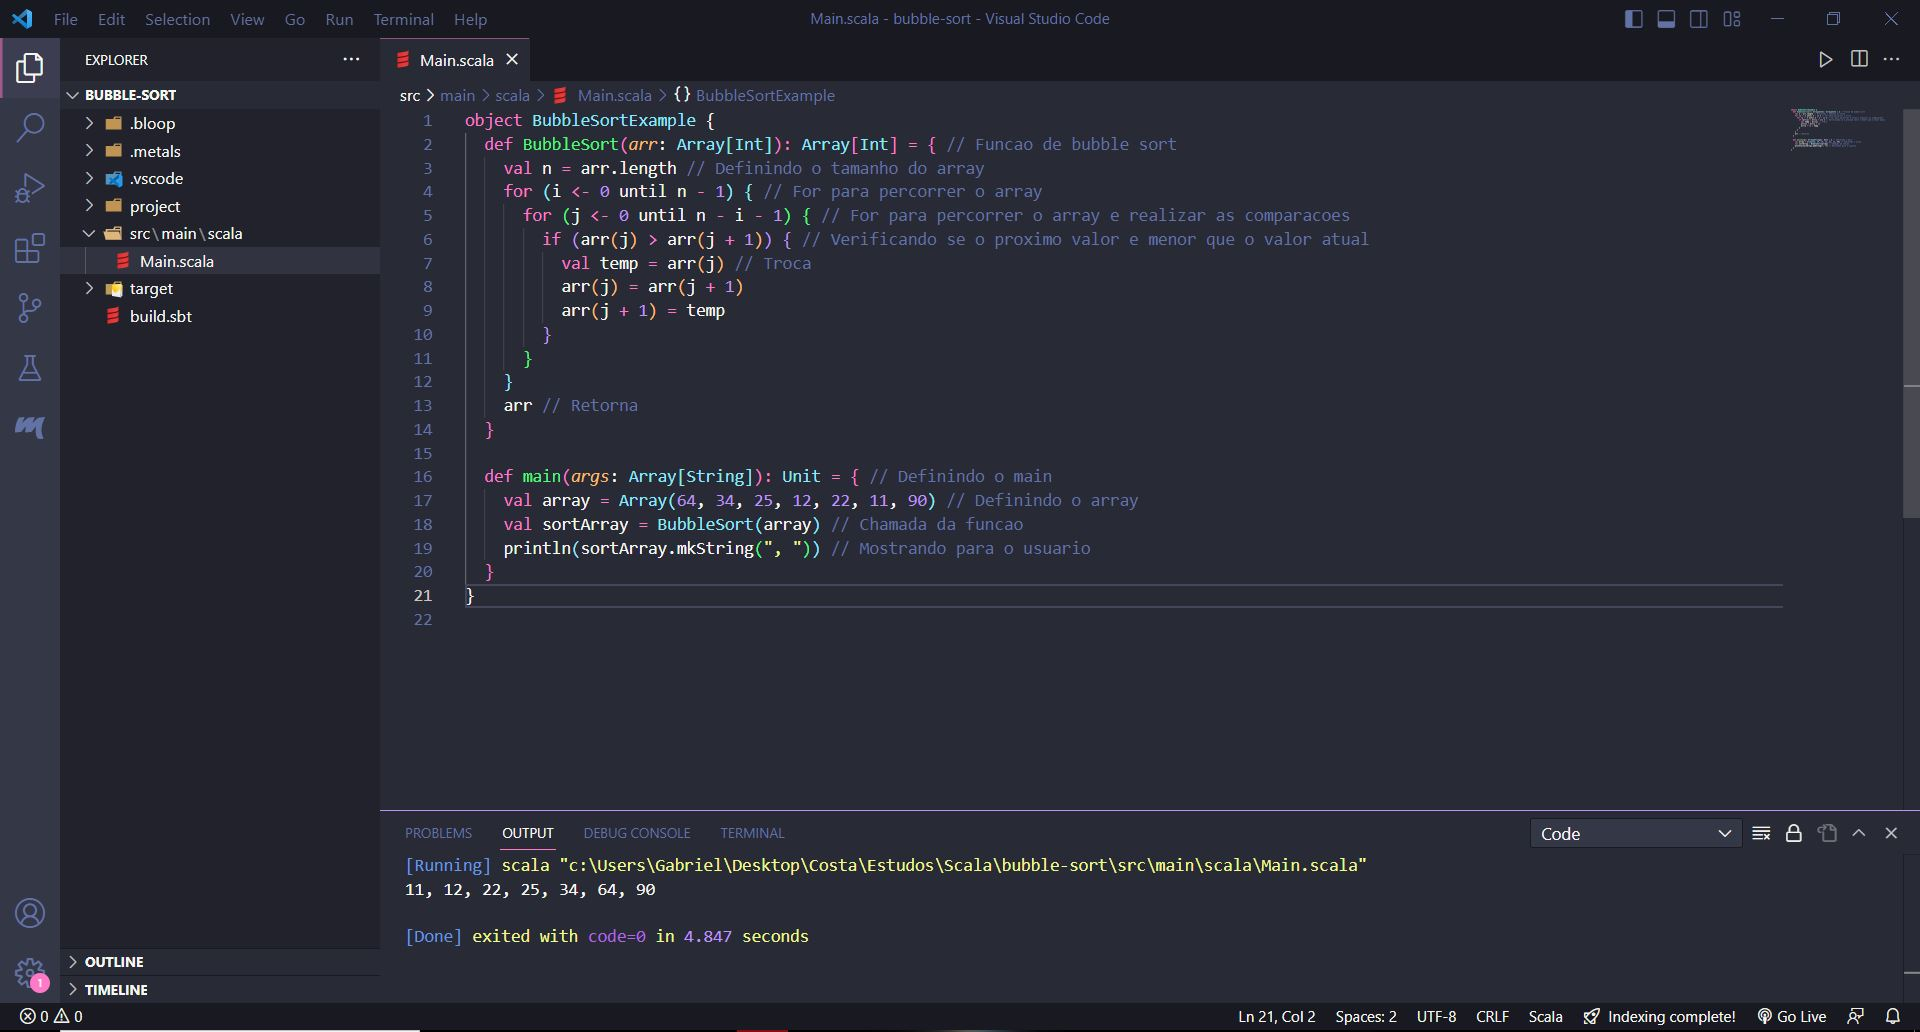
\includegraphics[width=17.5cm]{Pictures/Ferr1.1.jpg}
		\caption{}
		\label{fig:ferr1}
	\end{figure}
	
	\begin{figure}[H]
		\centering
		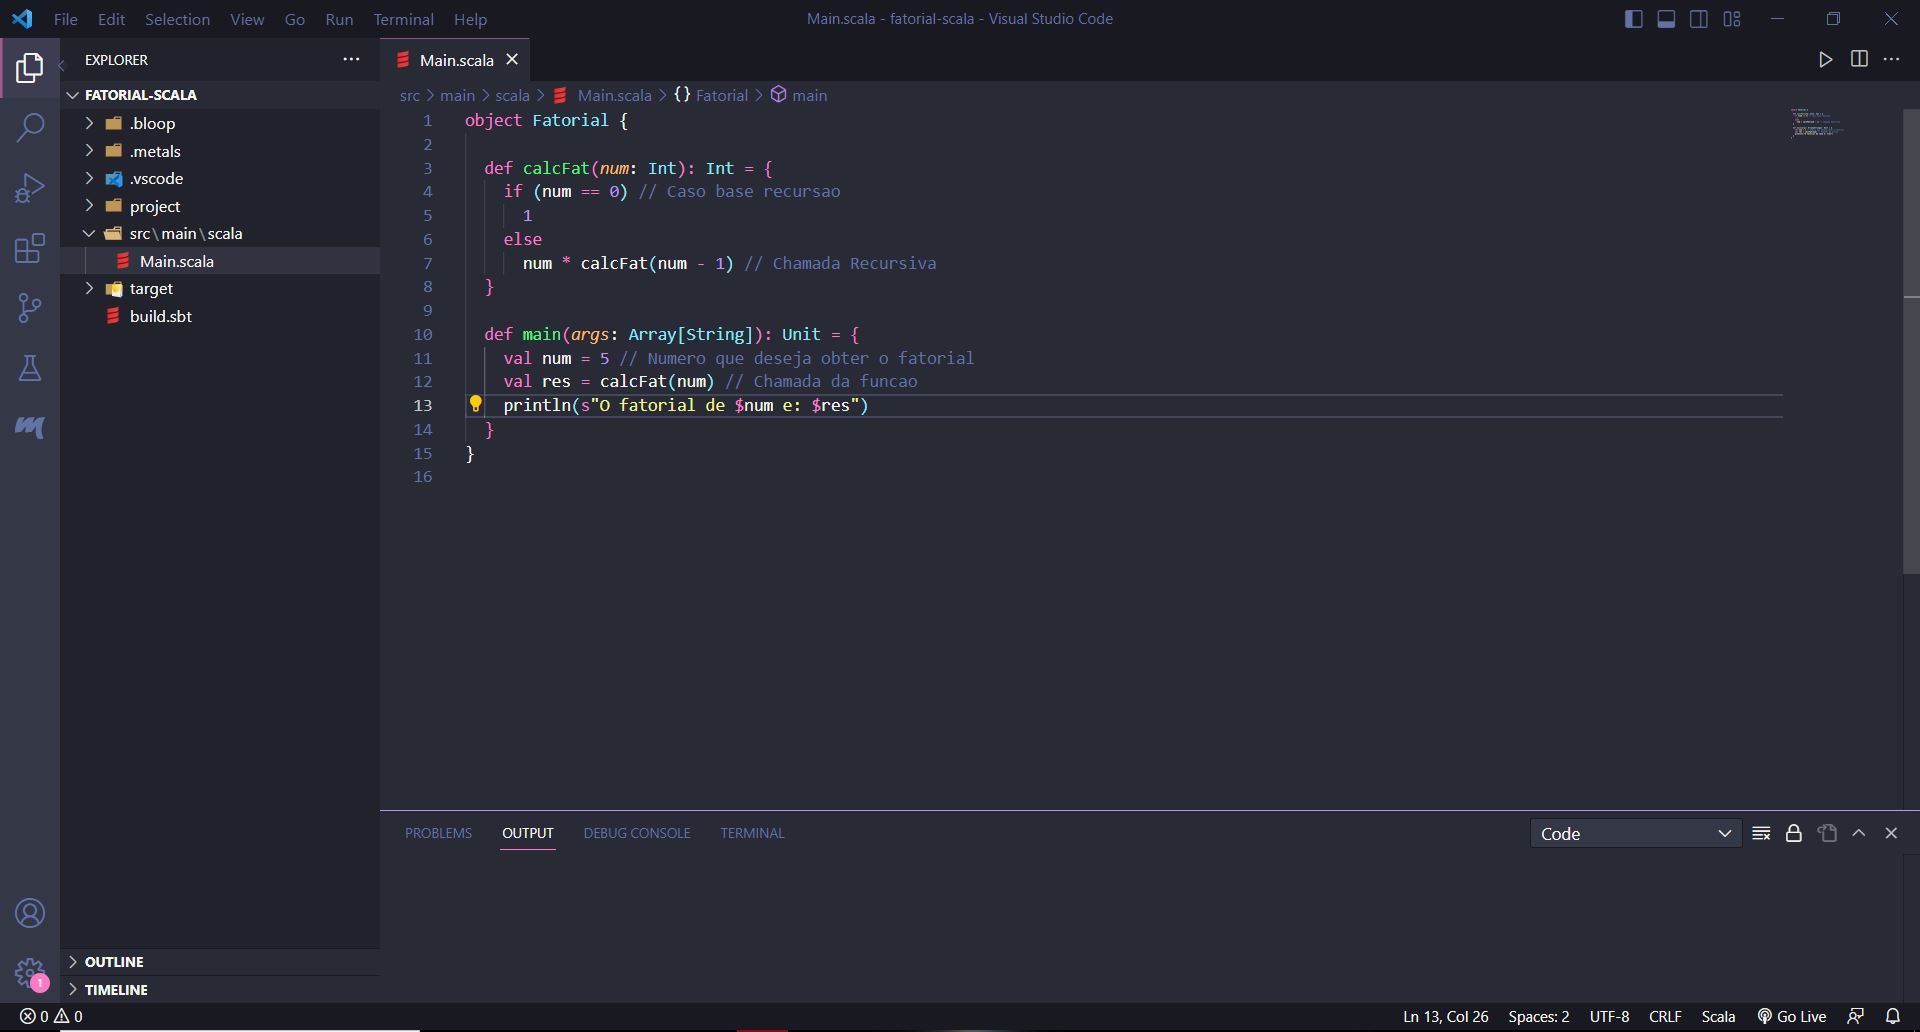
\includegraphics[width=17.5cm]{Pictures/Ferr1.2.jpg}
		\caption{}
		\label{fig:ferr2}
	\end{figure}

	\begin{figure}[H]
		\centering
		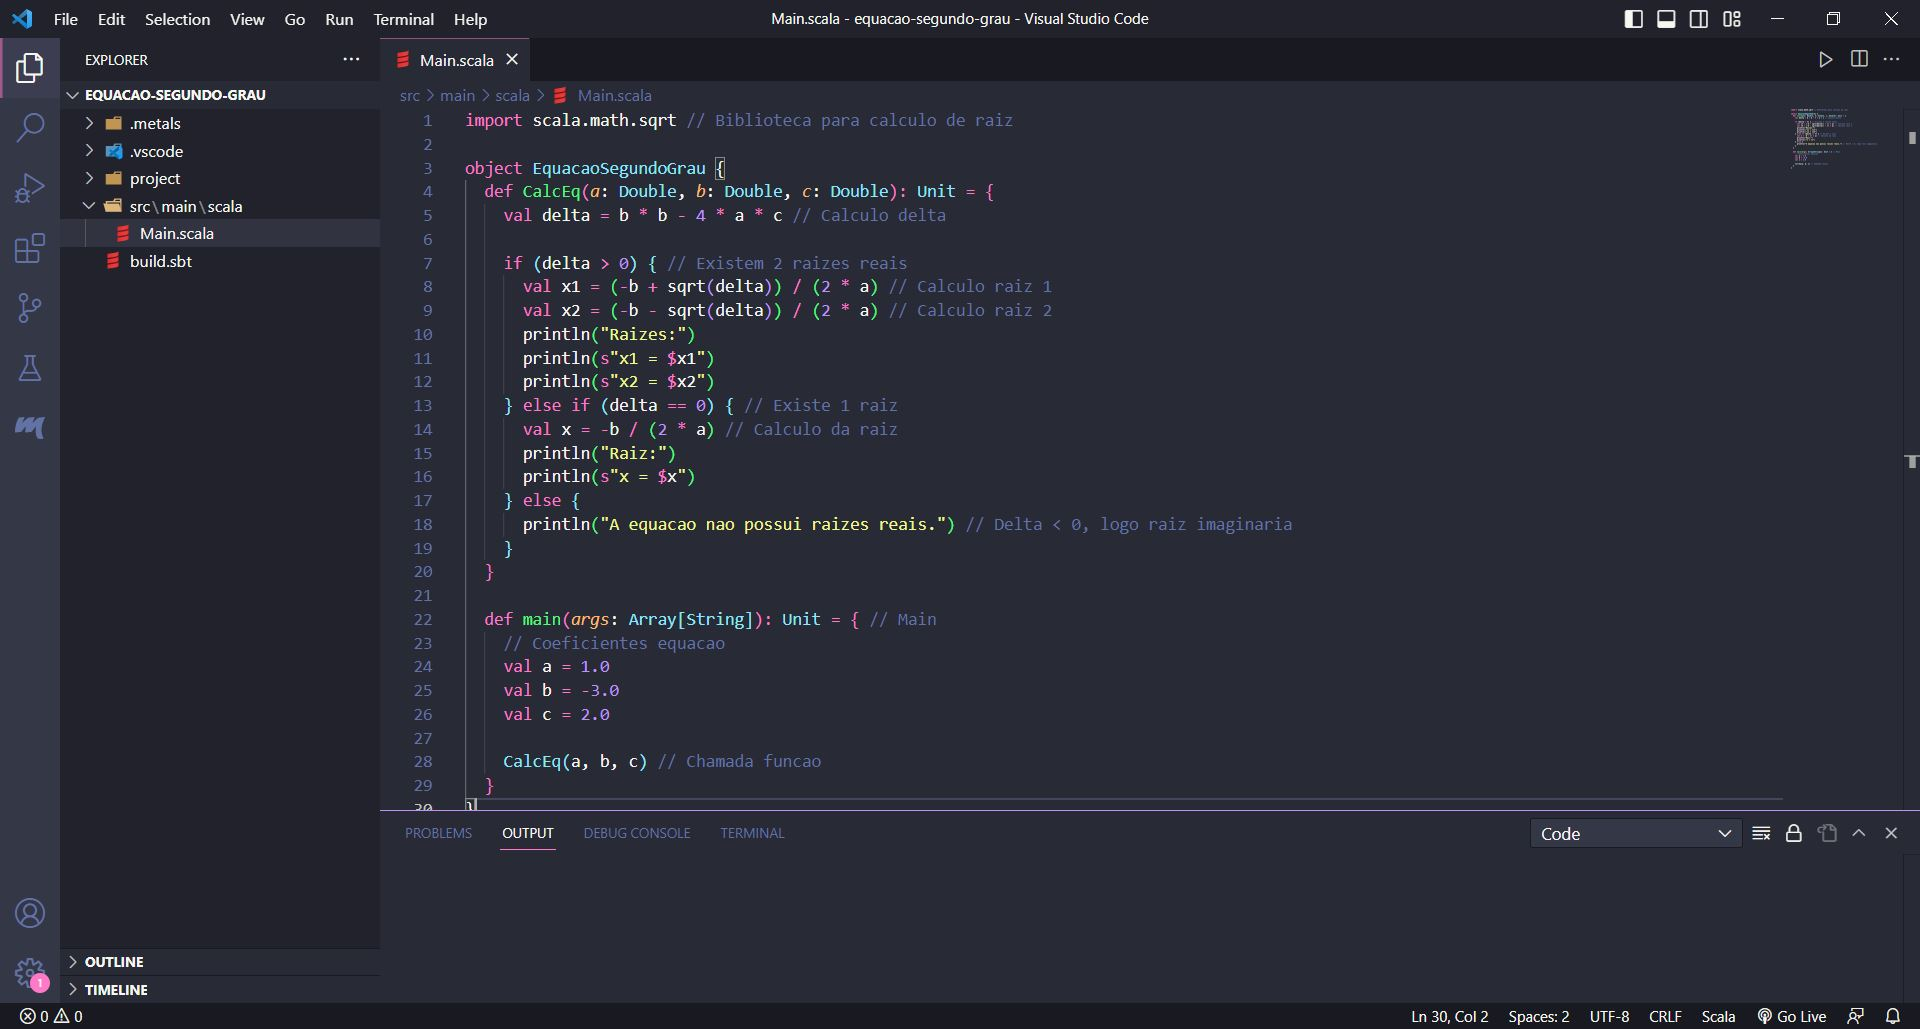
\includegraphics[width=17.5cm]{Pictures/Ferr1.3.jpg}
		\caption{}
		\label{fig:ferr3}
	\end{figure}

	Imagem da aba de extensões do VS Code: 
	\begin{figure}[H]
		\centering
		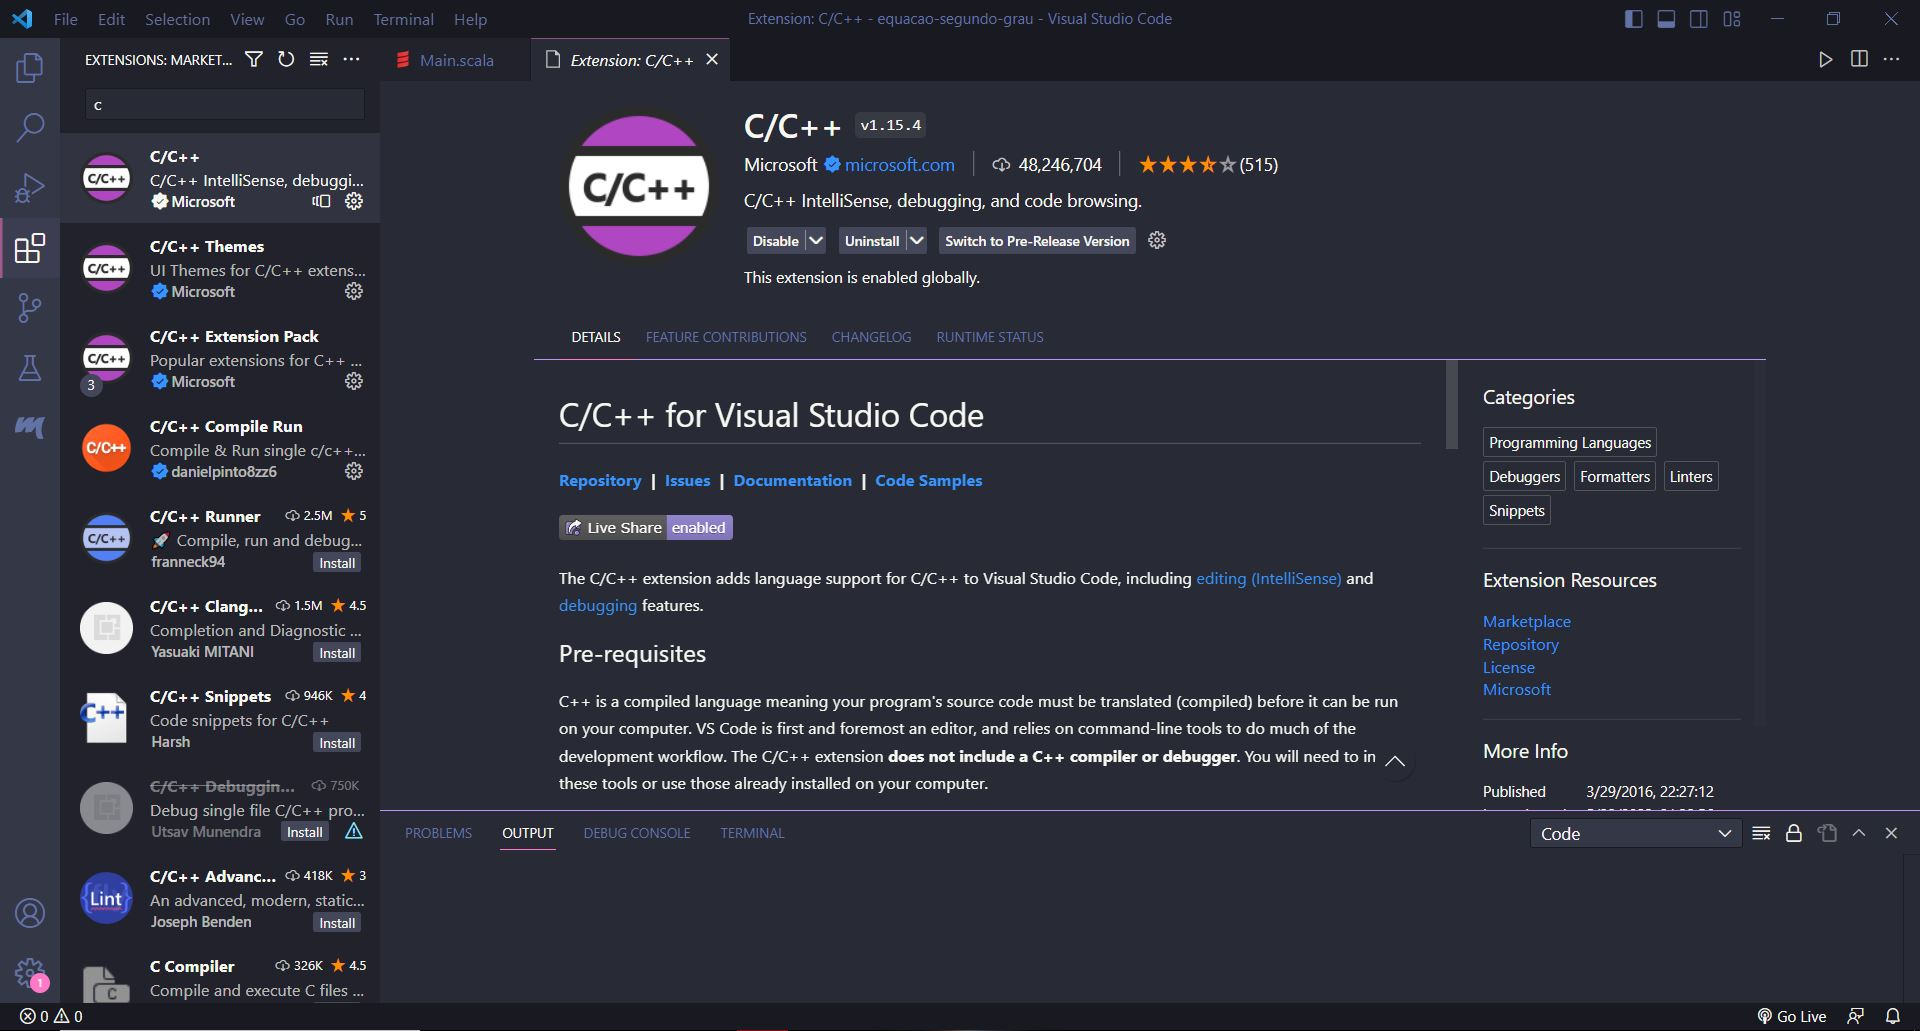
\includegraphics[width=17.5cm]{Pictures/Ferr1.4.jpg}
		\caption{}
		\label{fig:ferr4}
	\end{figure}
	

    \section{Scastie}
    O Scastie é uma plataforma online que permite executar código em Scala. É um ambiente de programação baseado na web criado com o intuito de ser de fácil acesso e interativo, e com o principal propósito: não precisar instalar nenhum software.
    
    Uma das características mais notáveis do Scastie é a capacidade de compartilhar códigos com outros usuários, facilitando a colaboração de diferentes programadores. Além disso, o ambiente de programação possibilita o usuário importar bibliotecas. Isso faz com que o Scastie seja uma ótima ferramenta para pessoas que desejam estudar, testar e compartilhar códigos em Scala.
    
    A ferramenta pode ser encontrada no próprio site do Scala ou clicando \href{https://scastie.scala-lang.org}{aqui}.
    
    \begin{figure}[H]
    	\centering
    	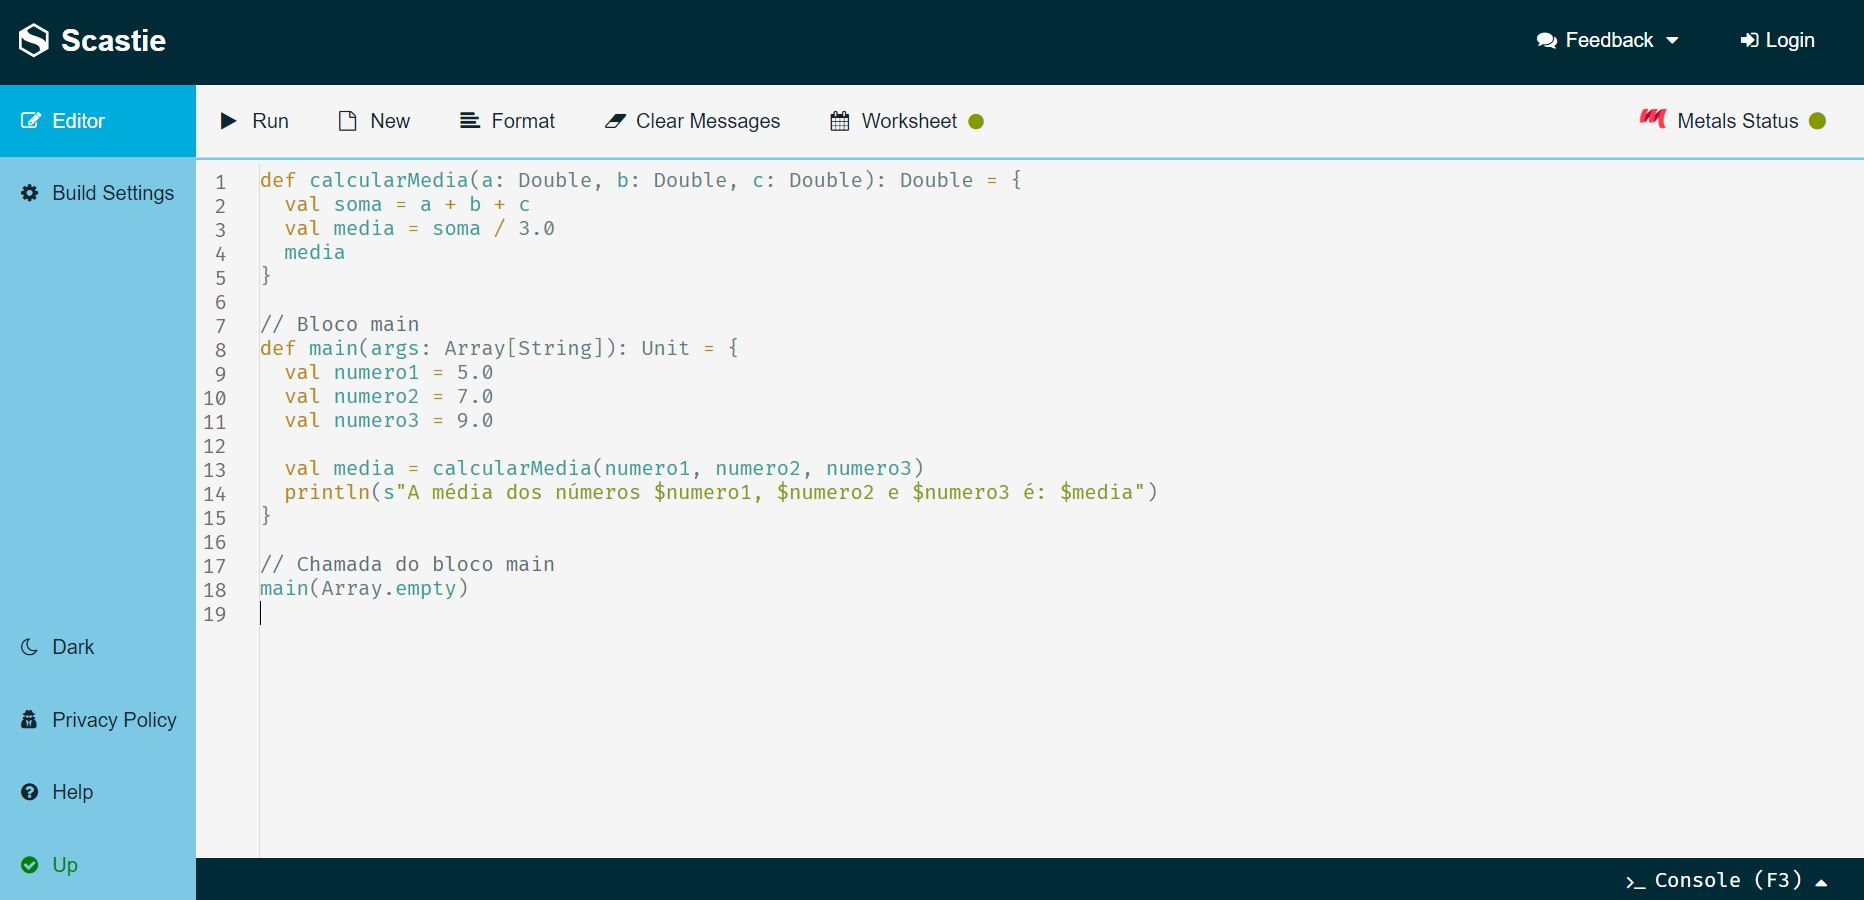
\includegraphics[width=17.5cm]{Pictures/Ferr2.1.jpg}
    	\caption{}
    	\label{fig:ferr1}
    \end{figure}

    \begin{figure}[H]
		\centering
		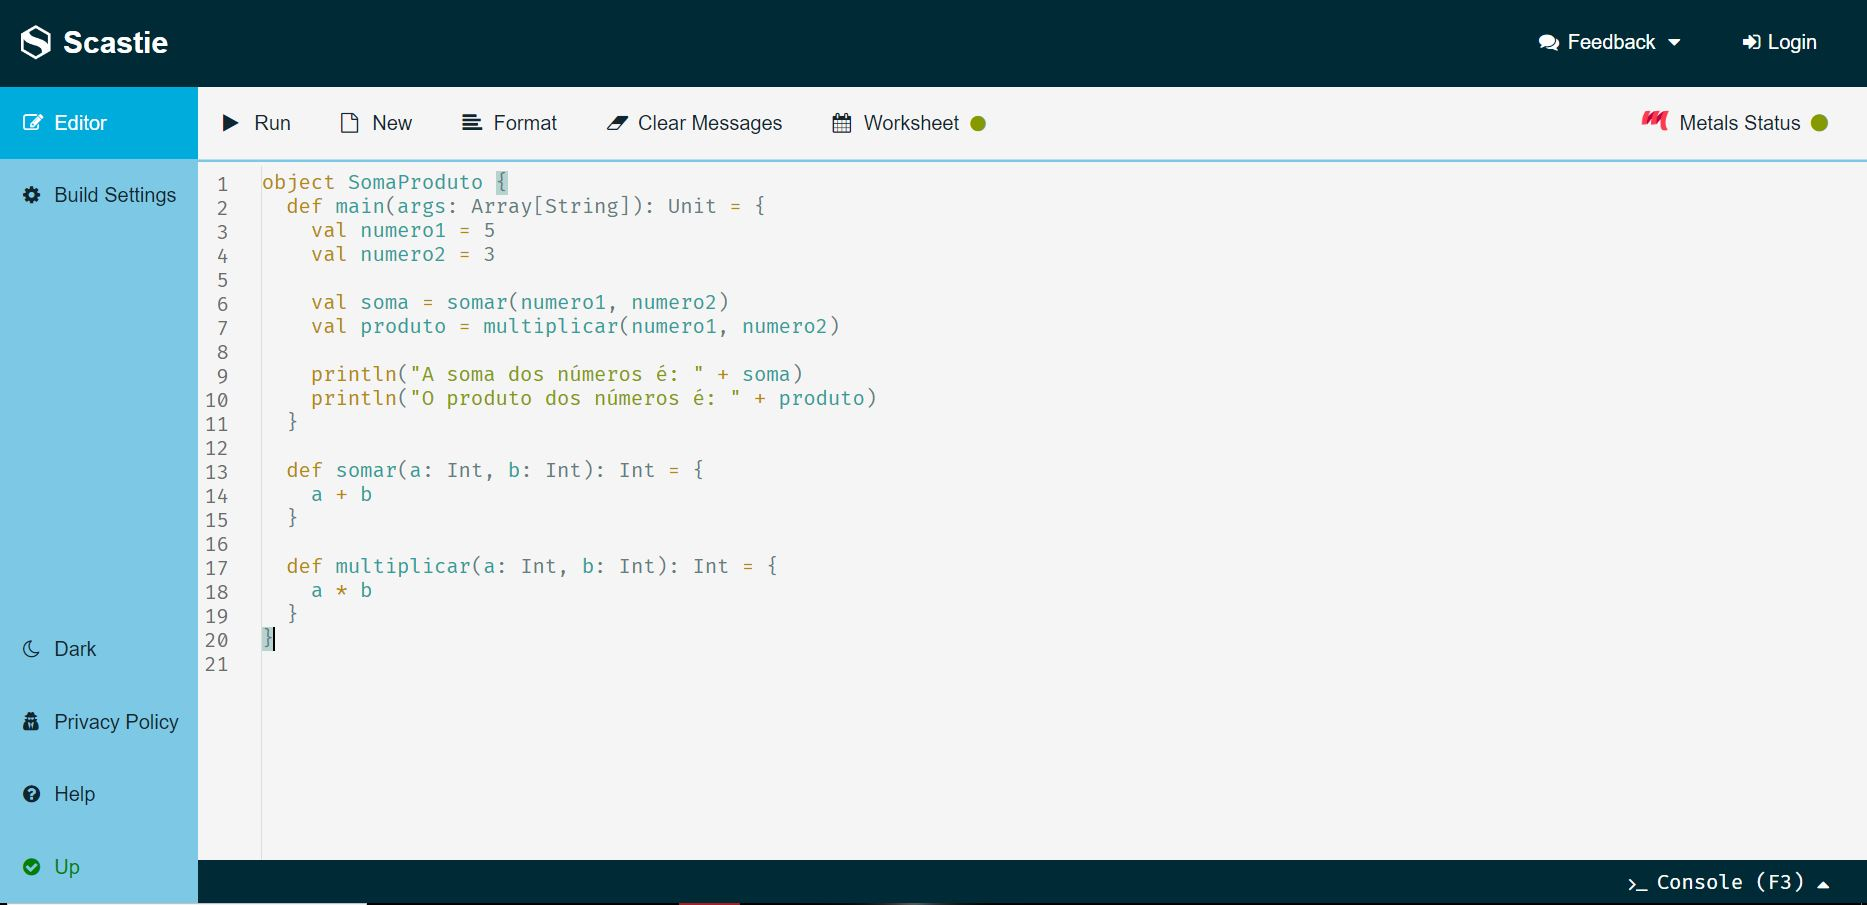
\includegraphics[width=17.5cm]{Pictures/Ferr2.2.jpg}
		\caption{}
		\label{fig:ferr2}
	\end{figure}

	\begin{figure}[H]
		\centering
		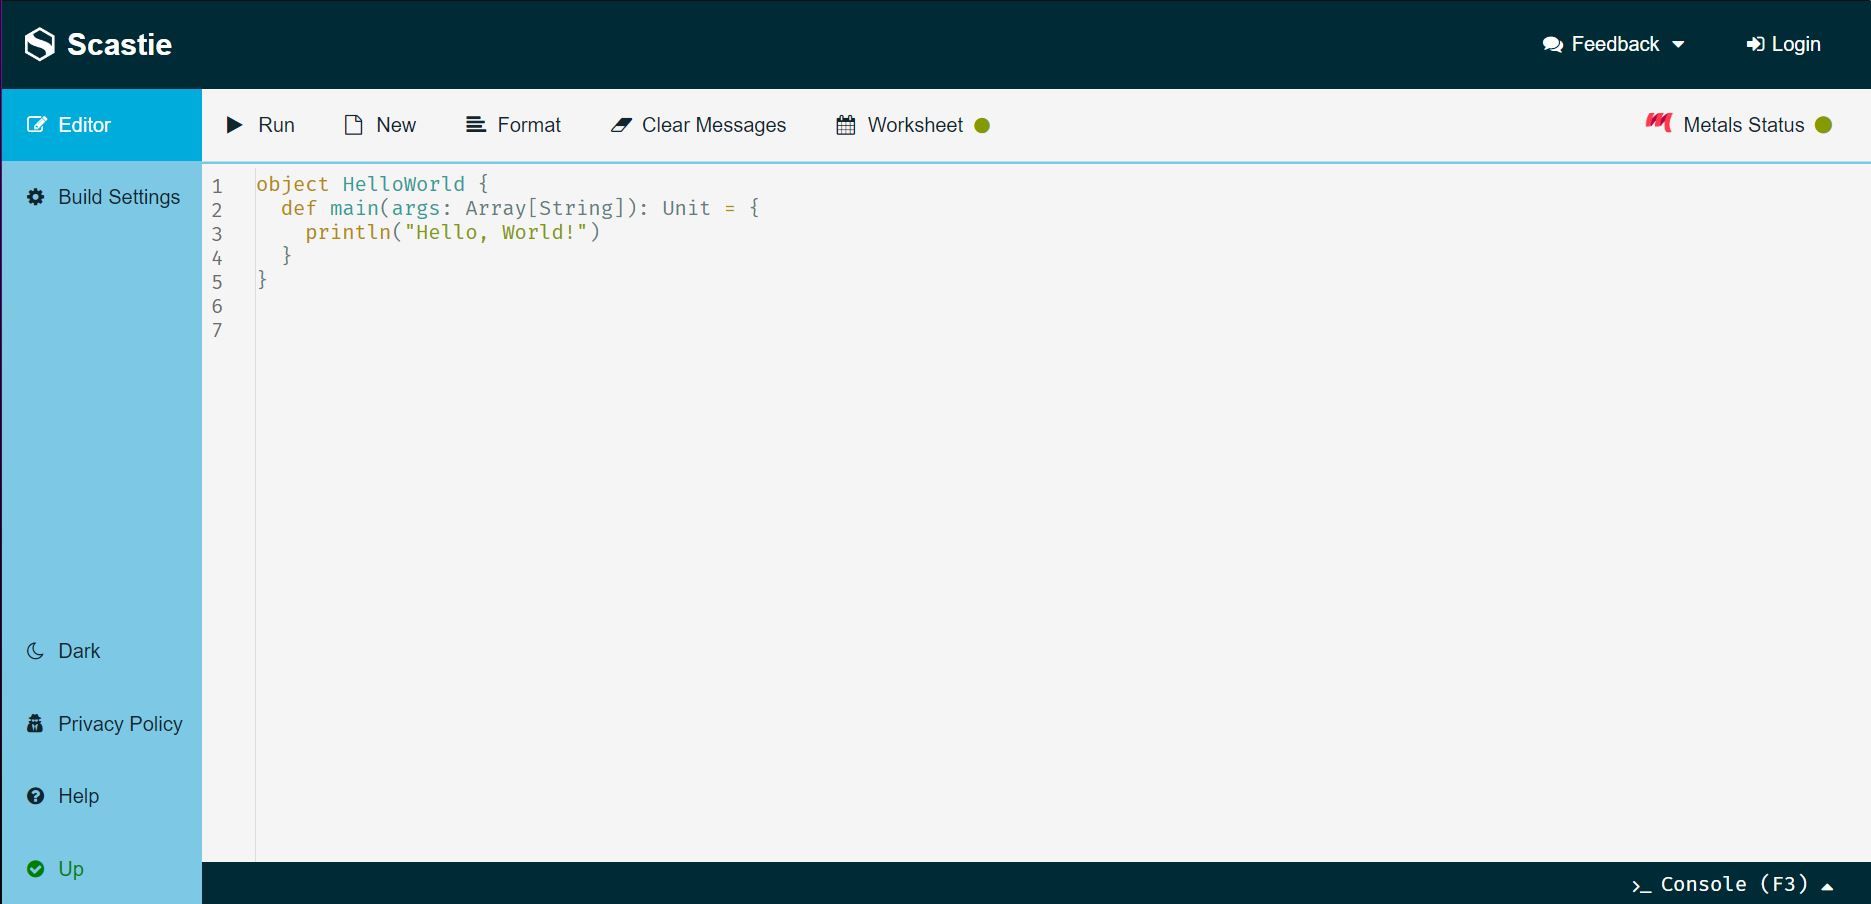
\includegraphics[width=17.5cm]{Pictures/Ferr2.3.jpg}
		\caption{}
		\label{fig:ferr3}
	\end{figure}





% Prof. Dr. Ausberto S. Castro Vera
% UENF - CCT - LCMAT - Curso de Ci\^{e}ncia da Computa\c{c}\~{a}o
% Campos, RJ,  2023
% Disciplina: Paradigmas de Linguagens de Programa\c{c}\~{a}o
% Aluno: Gabriel Costa Fassarella


\chapterimage{ScalaH} % Chapter heading image
\chapter{Considera\c{c}\~{o}es Finais}
	Ao longo desse livro foram abordados diversos aspectos sobre a linguagem de programação Scala. Inicialmente foi apresentada uma visão geral sobre a linguagem, seguido pela sua história que apesar de ser recente, não existem muitos relatos disponíveis para o público, e por último foram apresentadas algumas aplicações da linguagem no mercado de trabalho. 
	
	Após esse capítulo introdutório, foi abordado durante alguns capítulos aspectos básicos e avançados necessários para a programação em Scala. Em seguida foram demonstradas algumas aplicações utilizando esses conceitos apresentados anteriormente.
	
	É válido lembrar que esse livro foi escrito com o intuito de trazer uma introdução ao Scala junto com alguns necessários para a programação básica na linguagem, com o principal intuito de promover ao leitor o interesse de se aprofundar no estudo da linguagem Scala. 
	Aspectos do Scala que podem ser estudados futuramente:
	\begin{itemize}
		\item Traits e Mixins: Estudar o uso de traits com o objetivo de compartilhar os comportamentos entre classes e como compor traits pode ser algo vantajoso em muitas situações adversas.
		
		\item Programação Assíncrona: Estudar as bibliotecas Promises, Akka e Futures para poder utilizar paralelismo e concorrência de maneira efetiva pode garantir uma ótima eficiência do código.
		
		\item Macros: Estudar a utilização de macros para criar o código em tempo de compilação pode garantir muitas vantagens para o usuário.
		
		\item Implicits: Estudar o uso de implicits com o objetivo de adicionar comportamentos ou tipos implicitamente pode facilitar a utilização de inúmeras bibliotecas.
		
		\item Concorrência e Paralelismo: Como já citado antes, estudar o uso de paralelismo e a concorrência pode aumentar muito a eficiência do código em Scala.
		\end{itemize}

	Portanto, é possível concluir que o Scala é uma linguagem de programação extremamente versátil e útil e diversas áreas diferentes, tanto para o mercado de trabalho quanto para estudo. Isso, junto de sua similaridade com Java faz com que sua utilização tenha aumentado cada vez mais entre os programadores. Por isso, caso o leitor tenha o interesse em continuar ou reforçar os estudos na linguagem, são recomendados os seguintes livros:
	

   \begin{figure}[H]
    \begin{center}
        \caption{} \label{ling2}
        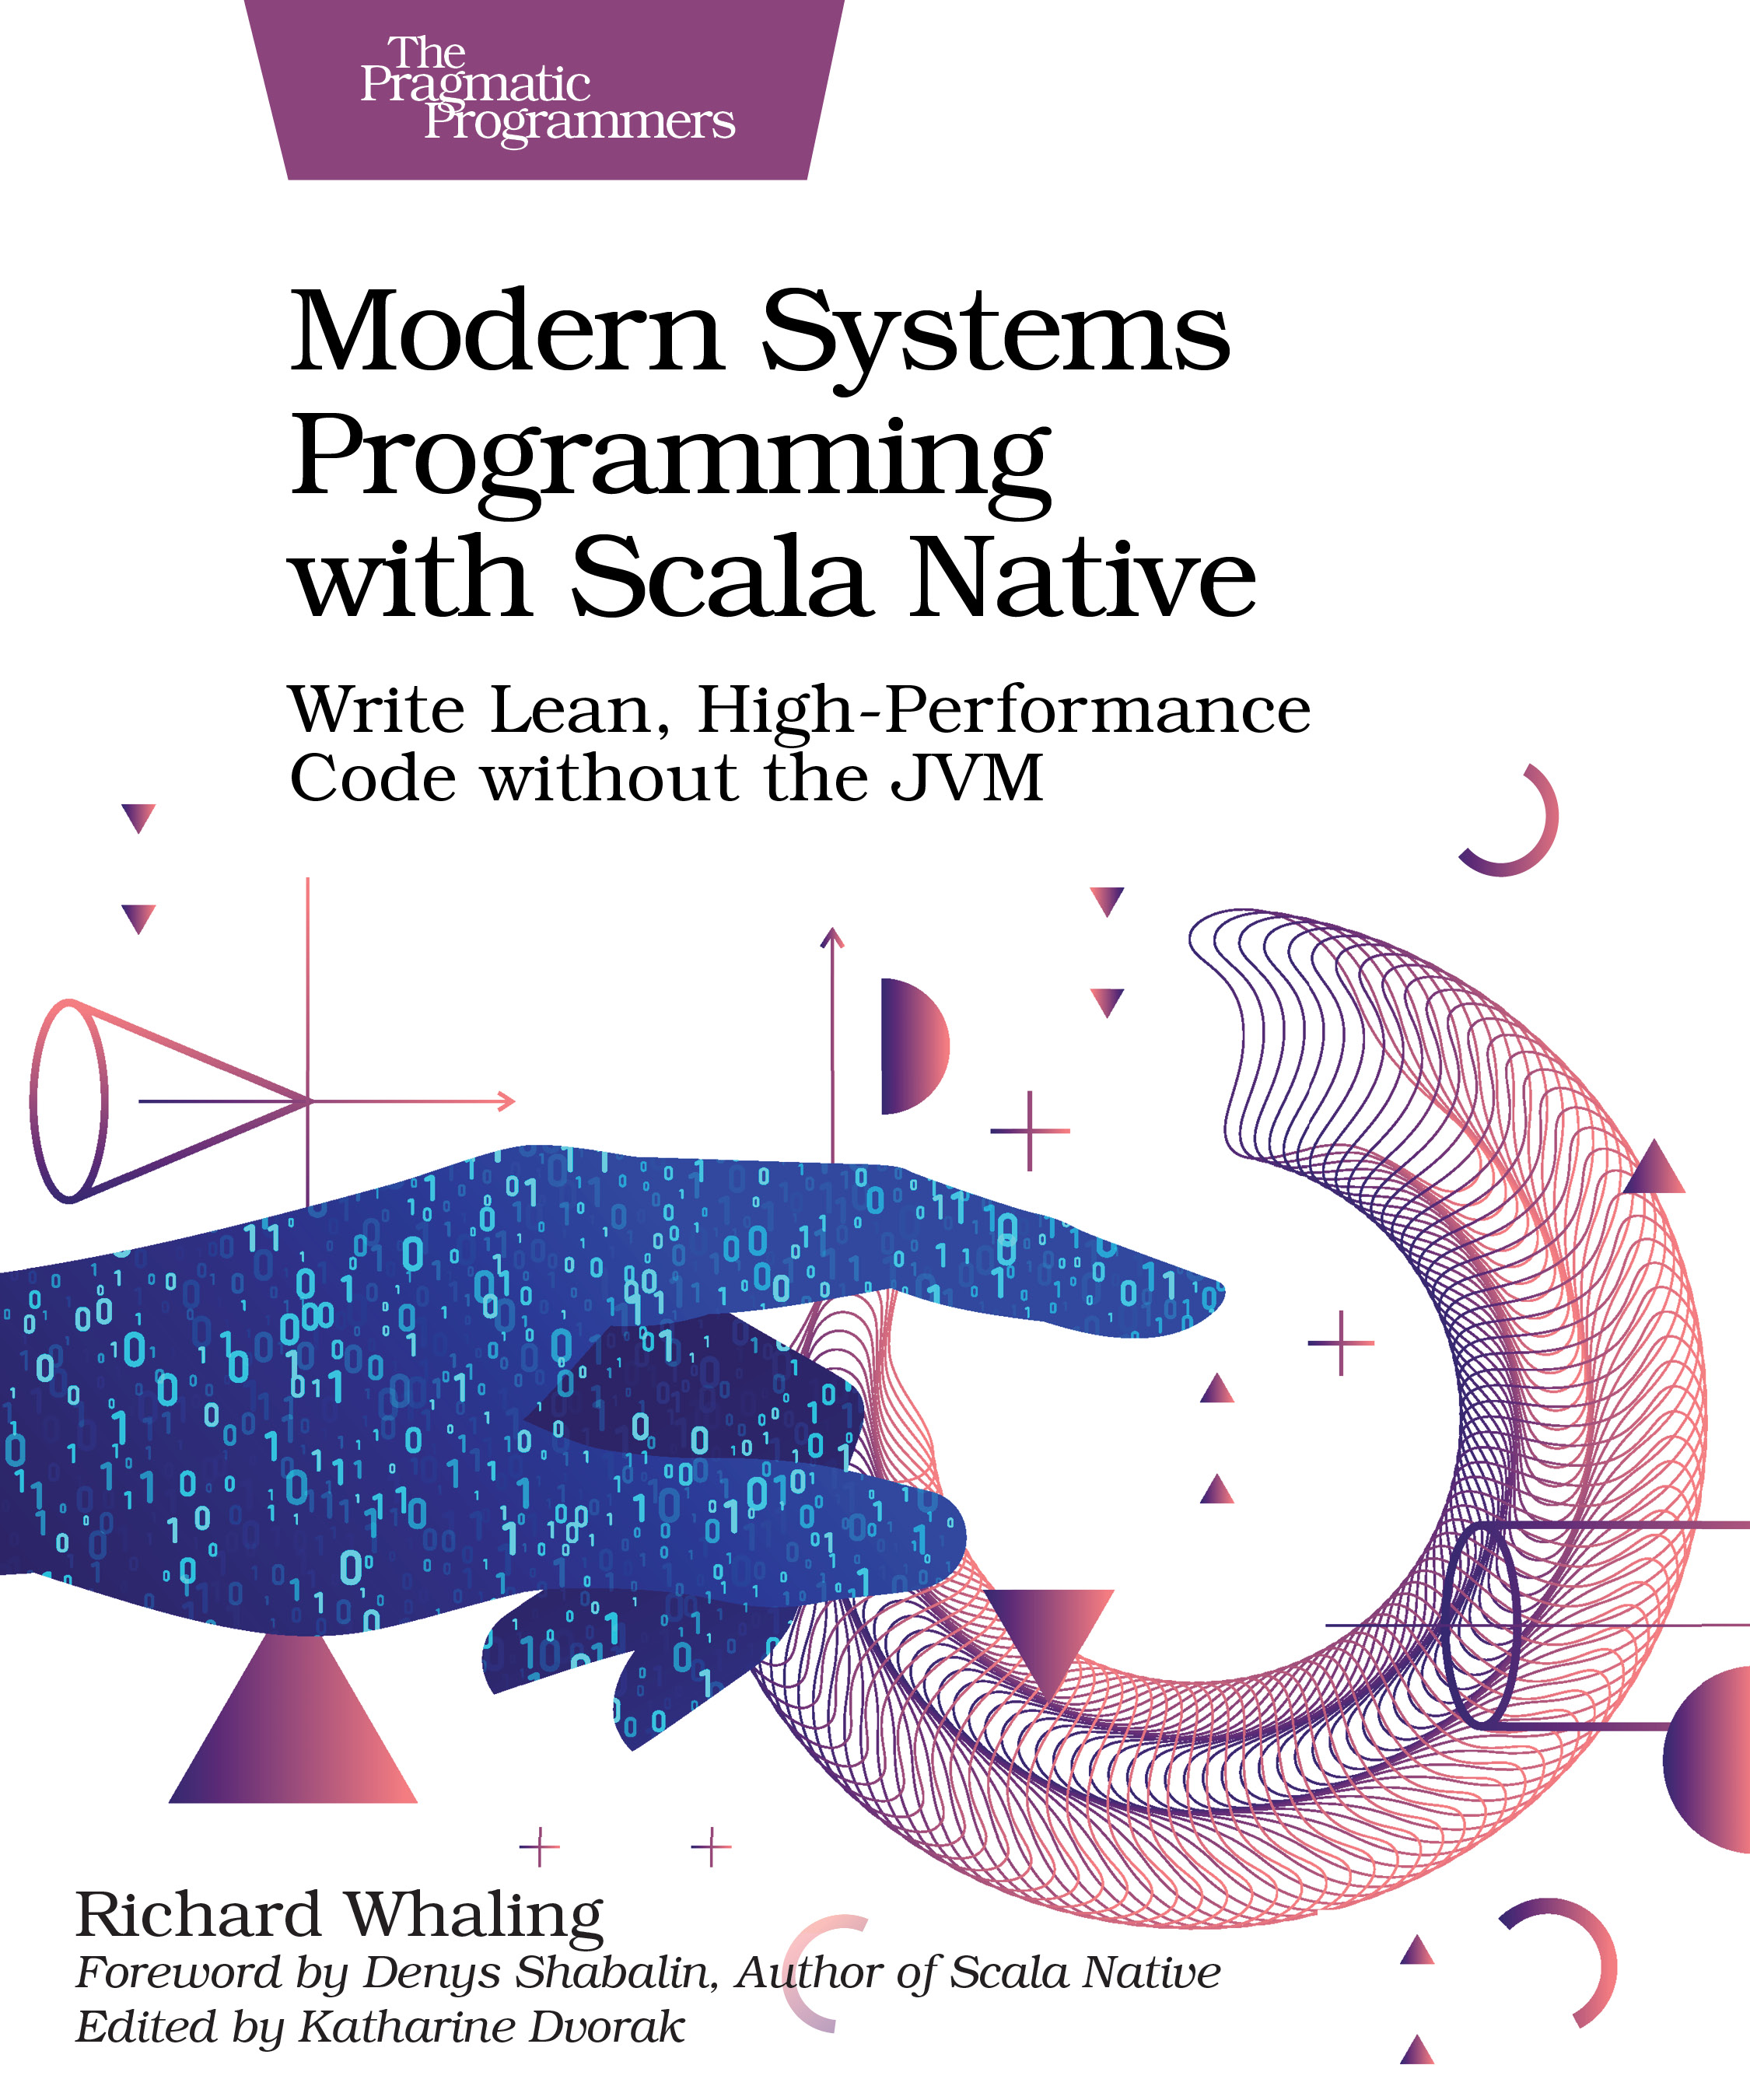
\includegraphics[width=7cm]{livro2020}
        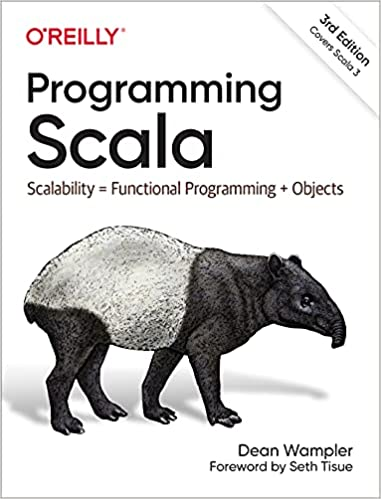
\includegraphics[width=7cm]{livro2021} \\
        {\tiny \sf Fonte: Autores }
    \end{center}
   \end{figure} 

	
	\begin{figure}[H]
		\centering
		
\includegraphics[width=7cm]{GetProgramming}
		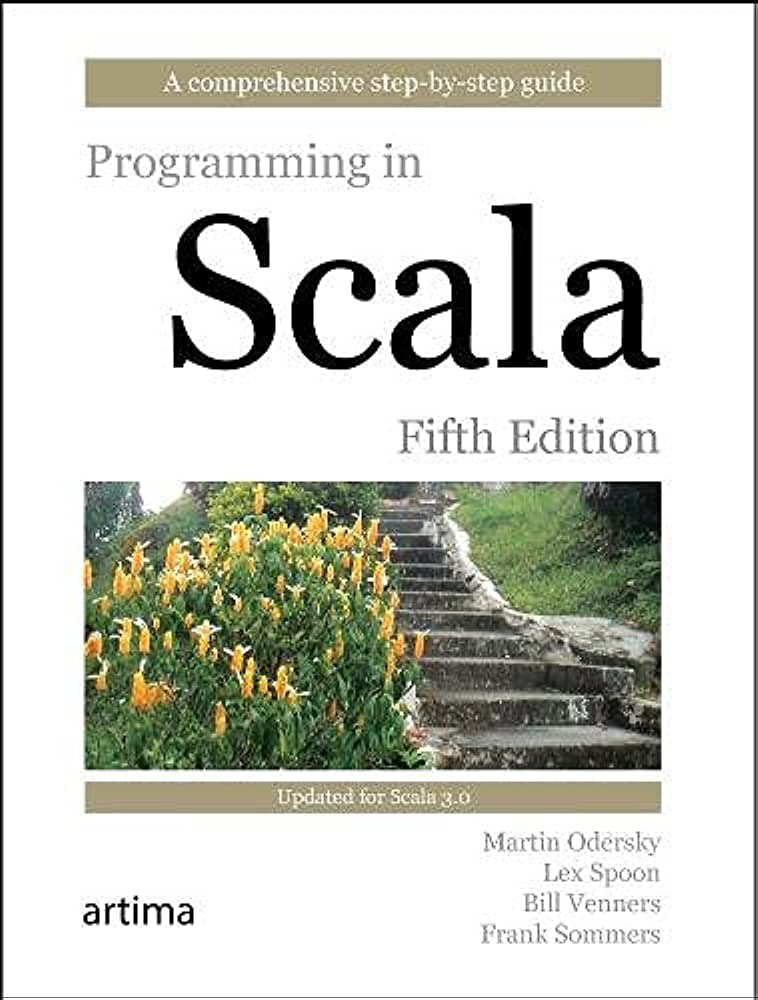
\includegraphics[width=7cm]{ProgrammingIn}
		\caption{}
		\label{fig:programming}
		Fonte: Autores
	\end{figure}

	\begin{figure}[H]
		\centering
		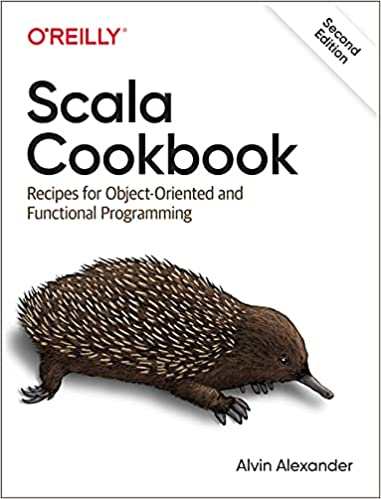
\includegraphics[width=7cm]{CookBook}
		\caption{}
		\label{fig:programming}
		Fonte: Autores
	\end{figure}

	










\chapterimage{Bibliografia.png}
\bibliographystyle{alpha}
\bibliography{Gabriel}
\addcontentsline{toc}{chapter}{\textcolor{ocre}{Bibliografia}}
%----------------------------------------------------------------------------------------
%	INDEX
%----------------------------------------------------------------------------------------

\cleardoublepage
\phantomsection
\setlength{\columnsep}{0.75cm}
\addcontentsline{toc}{chapter}{\textcolor{ocre}{Index}}
\printindex

%----------------------------------------------------------------------------------------

\end{document}

